\documentclass{article}
\usepackage[utf8]{inputenc}

% adjust top and bottom margin, https://www.ctan.org/pkg/geometry
\usepackage[top=1in, bottom=1in]{geometry}

% for serious mathematical typesetting, https://www.ctan.org/pkg/amsmath
\usepackage{amsmath}

% array and tabular environments, https://www.ctan.org/pkg/array
\usepackage{array}

% enhances the quality of tables, https://www.ctan.org/pkg/booktabs/
\usepackage{booktabs}

% improve the appearance of captions above tables
\usepackage{caption}

% use H to place figures and tables at exact location, https://www.ctan.org/pkg/float
\usepackage{float}

% manage images and define the images folder, https://ctan.org/pkg/graphicx
\usepackage{graphicx}
\graphicspath{{figures/}}

% create hyperlinks in the document and disable border, https://ctan.org/pkg/hyperref
\usepackage[hidelinks]{hyperref}

% use subfigure to place figures side-by-side, https://www.ctan.org/pkg/subcaption
\usepackage{subcaption}

% greek letters in text without math mode, https://www.ctan.org/pkg/textgreek
\usepackage{textgreek}

% change color of the text
\usepackage{xcolor}

% bibliography package and references file, https://www.ctan.org/pkg/biblatex
\usepackage[sorting=none]{biblatex}
\addbibresource{references.bib}

% Document
% ----------------------------------------------------------------------------

\title{Modeling Hydrodynamic and Biomass Pyrolysis Effects of Recycled Product Gases in a Bubbling Fluidized Bed Reactor}
\author{Gavin M. Wiggins, Oluwafemi A. Oyedeji, and Zachary G. Mills}
\date{\today}

\begin{document}

\maketitle

% Abstract
% ----------------------------------------------------------------------------

\section*{Abstract}

Fast pyrolysis of biomass in a fluidized bed reactor is typically conducted in a nitrogen gas environment. Recycling product gas can improve the economics of operating such a system by reducing reliance on pure process streams, but much less is known about how recycling pyrolysis product gas may affect fluidization behavior and pyrolysis kinetics. Therefore, gas effects in a fluidized bed biomass pyrolysis reactor were investigated using engineering correlations, low-order models, and CFD simulations for N$_2$, H$_2$, CO, CO$_2$, and CH$_4$ carrier gas mixtures. Our findings reveal viscosity of a gas mixture can be significantly underestimated depending on the model and correlation. Furthermore, fluidization characteristics such as U$_\textrm{mf}$ and gas-solid convective heat transfer can be greatly affected by the gas properties. \textcolor{blue}{By utilizing H$_2$ as the fluidizing gas (instead of N$_2$)}, while maintaining a constant fluidization ratio (U$_\text{s}$/U$_\text{mf}$), the bio-oil yields can be increased \textcolor{blue}{$\sim$5\%.} This is due to the lower density H$_2$ producing similar hydrodynamics as N$_2$ at higher gas flow rates. These higher flow rates result in shorter gas residence times, and as a result, less secondary reactions that convert bio-oil to light gases and char.

% Introduction
% ----------------------------------------------------------------------------

\section{Introduction}

Fast pyrolysis is a versatile method for thermochemical conversion of solid biomass into liquid bio-oil which can be used for bio-fuel and high-value chemical production. Several reactor types have been used for pyrolysis such as entrained flow, bubbling fluidized bed, fixed bed, auger, circulating fluidized bed, ablative, and spouted bed reactors \cite{Uddin-2018, Bridgwater-1991}. However, bio-oil derived from biomass feedstock is commonly generated in bubbling fluidized bed and circulating fluidized bed reactor systems in which biomass particles rapidly devolatilize in the absence of oxygen into mixtures of light gases, condensable bio-oil vapors, and solid char \cite{Bridgwater-1999, Bridgwater-2018a, Mohan-2006}. Since biomass pyrolysis normally occurs in a non-oxidizing environment, the fluidization gas (carrier gas) is often pure nitrogen \cite{Mohan-2006}. To maximize bio-oil yields, the reactor typically operates at temperatures near 500$^\circ$C and must maintain particle residence times up to 10 seconds and gas residence times less than 2 seconds \cite{Bridgwater-2018a}. Deviations from these conditions can result in significant production and quality penalties; therefore, optimal reactor design and control become crucial to achieving commercially viable bio-oil production.

To improve the economic feasibility of biomass fast pyrolysis systems, char can be burned for process heat while recycled pyrolysis gas can assist with fluidization \cite{Bridgwater-1999, Mante-2012, Elkasabi-2015}. The major generated components of pyrolysis gas are CO, CO$_2$, CH$_4$, H$_2$, along with other light hydrocarbons \cite{Asadullah-2008, Zhang-2011}. Experiments conducted by Mante et al. noticed increased liquid yields and decreased char/coke yields from fluidizing gas mixtures of CO/N$_2$, CO$_2$/N$_2$, CO/CO$_2$/N$_2$, and H$_2$/N$_2$ \cite{Mante-2012}. Mullen et al. recycled CO, CO$_2$, H$_2$ to create a reduced atmosphere in the reactor and saw deoxygenation effects on the pyrolysis oil along with lower total acid numbers and higher energy content \cite{Mullen-2013}. Zhang et al. investigated N$_2$, CO$_2$, CO, CH$_4$, and H$_2$ carrier gases and reported improved bio-oil heating value when using CO and H$_2$ as the carrier gas \cite{Zhang-2011}. Experiments by Elkasabi et al. recycled the non-condensable pyrolysis gas stream into the fluidized bed and noticed bio-oil with lower oxygen content and higher hydrocarbons compared to traditional bio-oil from an all nitrogen environment \cite{Elkasabi-2015}. Consequently, several experiments have studied the effects of different fluidization gases on pyrolysis yields but modeling these effects was not discussed in the reported literature.

Autothermal pyrolysis experiments in a fluidized bed reactor has shown that the presence of oxygen in the carrier gas can prevent reactor clogging by reducing char formation \cite{Kim-2014}. The addition of oxygen can also improve heat transfer within the reactor via partial oxidiation of the pyrolysis products without significant decreases in bio-oil yield \cite{Polin-2019a, Oyedeji-2022}. Substituting air for nitrogen gas allowed for higher superficial velocities which promoted elutriation of char from reactor experiments while having neglible effect on bio-oil yield \cite{Polin-2019b}. Modeling the fluidization behavior inside the reactor at autothermal pyrolysis conditions was not discussed in the available literature.

There are several fluidized bed reactor models that investigate the hydrodynamics and conversion of biomass at fast pyrolysis conditions \cite{Papadikis-2009, Papadikis-2010, Mellin-2014, Xiong-2016, Xue-2011}. These models assume the carrier gas is pure nitrogen which is a typical scenario for biomass fast pyrolysis. We are not aware of any models in the biomass pyrolysis literature that investigate the effects of a carrier gas other than pure nitrogen. Consequently, our objective in this paper is to evaluate different fluidization gases and their effects on the hydrodynamics and biomass conversion in a bubbling fluidized bed reactor operating at fast pyrolysis conditions. Modeling the effects on the pyrolysis reaction chemistry is not possible because current kinetic schemes for biomass pyrolysis do not account for carrier gas properties. Our methodology uses engineering correlations, reducing-order modeling techniques, and CFD simulations to model these effects and compare the model results (where applicable) to experimental data.

% Experimental apparatus
% ----------------------------------------------------------------------------

\section{Experimental apparatus}

The NREL 2FBR reactor system thermochemically converts biomass feedstock at fast pyrolysis conditions. The system is comprised of a bubbling fluidized bed (BFB) reactor known as the ``pyrolyzer''. An overview of the components and inlet/outlet flows of the NREL 2FBR pyrolysis unit is shown in Figure \ref{fig:pyrolyzer-components}, while dimensions and typical operating conditions of the pyrolysis reactor are detailed in Figure \ref{fig:pyrolyzer-dims-flows}. Sand along with the carrier gas is used as the fluidization medium in the pyrolyzer while biomass particles are fed to the reactor via a screw auger. More information about the NREL 2FBR biomass pyrolysis system is available elsewhere \cite{Howe-2015, Trendewicz-2015}. Yields from the BFB pyrolysis reactor are compared to model results discussed later in this paper.

\begin{figure}[H]
    \centering
    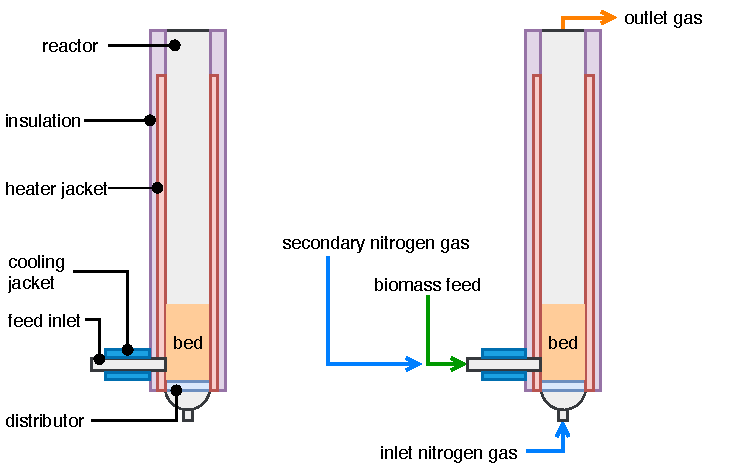
\includegraphics[width=0.8\textwidth]{pyrolyzer-components.pdf}
    \caption{Components (left) and inlet/outlet flows (right) for the BFB biomass pyrolysis reactor in the NREL 2FBR system.}
    \label{fig:pyrolyzer-components}
\end{figure}

\begin{figure}[H]
    \centering
    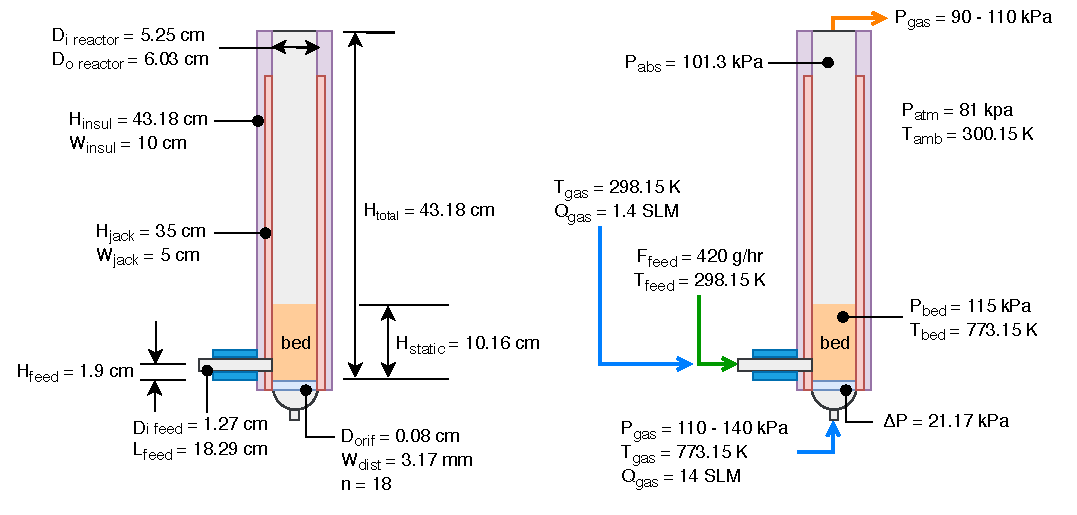
\includegraphics[width=\textwidth]{pyrolyzer-dims-flows.pdf}
    \caption{Dimensions (left) and typical fast pyrolysis operating conditions (right) for the BFB biomass pyrolysis reactor in the NREL 2FBR system.}
    \label{fig:pyrolyzer-dims-flows}
\end{figure}

% Modeling approach
% ----------------------------------------------------------------------------

\section{Modeling approach}

Our strategy to model and understand gas effects in a bubbling fluidized bed reactor begins with determining gas properties such as density, dynamic viscosity, thermal conductivity, and heat capacity. Once the individual gas viscosity is known, the viscosity of a gas mixture is calculated using various mixture models. Next, fluidization correlations relevant to fluidized bed reactors are used to investigate the effects of the gas properties on the hydrodynamics of the system. Dimensionless numbers provide insight on the limiting mechanisms in regards to the pyrolysis of the biomass particles. Finally, CFD-DEM simulations provide residence times and product yields related to the different carrier gas scenarios.

\subsection{Gas properties}

Dynamic gas viscosity $\mu_\text{gas}$ is estimated by Equation \ref{eq:viscosity} in units of \textmugreek P. Gas thermal conductivity k$_\text{gas}$ as W/m$\cdot$K is calculated from Equation \ref{eq:thermlcond} and heat capacity C$_\text{p\,gas}$ as J/mol$\cdot$K is determined using Equation \ref{eq:heatcap}. In each equation, temperature is denoted by T in units of Kelvin while the regression coefficients A, B, C, D, E, F, and G for a particular gas were obtained from Yaws' Handbook for each gas property \cite{Yaws2014}.

\begin{equation}\label{eq:viscosity}
    \mu_\text{gas} = A + B\,T + C\,T^2 + D\,T^3
\end{equation}

\begin{equation}\label{eq:thermlcond}
    k_\text{gas} = A + B\,T + C\,T^2 + D\,T^3
\end{equation}

\begin{equation}\label{eq:heatcap}
    C_\text{p\,gas} = A + B\,T + C\,T^2 + D\,T^3 + E\,T^4 + F\,T^5 + G\,T^6
\end{equation}

Several methods are available to calculate the dynamic viscosity of a gas mixture. The simplest approach is Graham's model in Equation \ref{eq:graham} which calculates the mixture viscosity from the mole weighted average of the component viscosities \cite{Graham-1846}.

\begin{equation}
    \mu_\text{mix} = \sum(x_i \; \mu_i)
    \label{eq:graham}
\end{equation}

\noindent The Herning and Zipperer approach shown by Equation \ref{eq:herning}, sums the viscosities weighted by the square root of the molecular weight M$_\text{i}$ for each component \cite{Herning-1936}. According to Davidson's report \cite{Davidson-1993}, the Herning and Zipperer model is not recommended for gas mixtures containing significant amounts of hydrogen.

\begin{equation}
    \mu_\text{mix} = \sum \frac{\mu_i \; x_i \; \sqrt{M_i}}{x_i \; \sqrt{M_i}}
    \label{eq:herning}
\end{equation}

\noindent Wilke's model represented by Equations \ref{eq:wilke-phi} and \ref{eq:wilke-mu} is based on a kinetic theory implementation which requires a coefficient $\phi_\text{ij}$ for each gas component \cite{Wilke-1950}. The coefficients are used along with the mole fractions to calculate the overall mixture viscosity.

\begin{align}
    \phi_{ij} &= \frac{\left[1 + (\mu_i/\mu_j)^{1/2} (M_j/M_i)^{1/4}\right]^2}{(4/\sqrt{2}) \left[1 + (M_i/M_j)\right]^{1/2}} \label{eq:wilke-phi} \\
    \mu_{\text{mix}} &= \sum_{i=1} \frac{\mu_i}{1 + \frac{1}{x_i} \sum_{\substack{j=1 \\j \neq i}} x_j \, \phi_{ij}} \label{eq:wilke-mu}
\end{align}

\noindent Brokaw provides a model for nonpolar and polar gas mixtures that utilizes the viscosities, molecular weights, and mole fractions of the mixture components \cite{Brokaw-1968}. The molecular weight ratios of the gas components are described by Equations \ref{eq:brokaw-mij} and \ref{eq:brokaw-aij}; the ratios are used in Equation \ref{eq:brokaw-mu} to calculate the overall mixture viscosity where S$_\text{ij} = 1$ for nonpolar gases.

\begin{align}
    m_{ij} &= \left[ 4 M_i M_j / (M_i + M_j)^2 \right]^{1/4} \label{eq:brokaw-mij} \\
    A_{ij} &= m_{ij}\left( \frac{M_j}{M_i} \right)^{1/2} \left[ 1 + \frac{\frac{M_i}{M_j} - \left(\frac{M_i}{M_j} \right)^{0.45} }{ 2 \left(1 + \frac{M_i}{M_j} \right) + \frac{1 + \left(\frac{M_i}{M_j} \right)^{0.45}}{1 + m_{ij}} m_{ij}} \right] \label{eq:brokaw-aij} \\
    \mu_{\text{mix}} &= \sum_{i=1} \frac{x_i \sqrt{\mu_i}}{\frac{x_i}{\sqrt{\mu_i}} + \sum_{\substack{j=1 \\ j \neq i}} \frac{S_{ij} \, A_{ij}}{\sqrt{\mu_j}} x_j} \label{eq:brokaw-mu}
\end{align}

\noindent Lastly, the approach by Davidson estimates viscosity in terms of the fluidity of the gas mixture \cite{Davidson-1993}. This method utilizes the momentum efficiency of the gas components to predict the mixture fluidity which is the reciprocal of the gas viscosity as given by Equations \ref{eq:davidson-eij}, \ref{eq:davidson-f}, and \ref{eq:davidson-mu} respectively. The empirical constant A was calculated as 0.375 using reported viscosities of 35 gas pairs \cite{Davidson-1993}.

\begin{align}
    E_{ij} &= \frac{2 \sqrt{M_i\, M_j}}{M_i + M_j} \label{eq:davidson-eij} \\
    f &= \sum \frac{x_i\, x_j}{\sqrt{\mu_i\, \mu_j}} E_{ij}^A \label{eq:davidson-f} \\
    \mu_\text{mix} &= 1 / f \label{eq:davidson-mu}
\end{align}

\subsection{Fluidization correlations}

For a bed of particles, the minimum fluidization velocity U$_\text{mf}$ is the gas velocity at which the drag force of the upward moving gas equals the weight of the particles. Kunii and Levenspiel \cite{Levenspiel-1991} provide the following equation for calculating minimum fluidization velocity

\begin{equation}
    U_\text{mf} = \frac{Re_\text{p,mf}\; \mu}{d_p\, \rho_g}
\end{equation}

\noindent where $\mu$ is gas viscosity (kg/m$\cdot$s), d$_\text{p}$ is particle diameter (m), $\rho_\text{g}$ is gas density (kg/m$^3$), and Re$_\text{p,mf}$ is the particle Reynolds number at minimum fluidization conditions. The Reynolds number is calculated using the Archimedes number (Ar) as follows

\begin{align}
    Re_{p,mf} &= \left( a^2 + b Ar \right)^{1/2} - a \\
    Ar &= \frac{d_p^3 \rho_g (\rho_s - \rho_g) g}{\mu^2}
\end{align}

\noindent where a and b are dimensionless constants which represent experimental coefficients. Some U$_\text{mf}$ correlations in the literature are based on experimental data from Wen and Yu where a, b = 33.7, 0.0408; from Richardson where a, b = 25.7, 0.0365; and from Grace where a, b = 27.2, 0.0408 \cite{Levenspiel-1991}. However, Kunii and Levenspiel \cite{Levenspiel-1991} suggest the constants ($a, b$) can be derived from the Ergun pressure drop equation based on constants K$_1$ and K$_2$ where $\epsilon_\text{mf}$ is the bed void fraction at minimum fluidization and $\phi$ is sphericity of the bed particles. For this paper, U$_\text{mf}$ is estimated based on the Ergun, Grace, Richardson, and Wen and Yu correlations.

\begin{equation}
    a = \frac{K_2}{2 K_1} \qquad
    b = \frac{1}{K_1}
\end{equation}

\begin{equation}
    K_1 = \frac{1.75}{\epsilon_{mf}^3 \phi} \qquad
    K_2 = \frac{150(1-\epsilon_{mf})}{\epsilon_{mf}^3 \phi^2}
\end{equation}

The terminal velocity U$_\text{t}$ of a particle is the minimum gas velocity to entrain a particle of size d$_\text{p}$. This velocity can be estimated from the maximum velocity of a particle in free-fall through a fluid, which is given by Equation \ref{eq:terminal}. Here, Re$_\text{p}$ is the particle Reynolds number given by Equation \ref{eq:particleRe} and C$_\text{D}$ is the drag coefficient which was estimated from an emperical correlation developed by Haider and Levenspiel \cite{haider1989drag} and given by Equation \ref{eq:dragCoeff}.

\begin{align}
    U_{t} &= \left [\frac{4d_{p} \left (\rho_{s}-\rho_{g} \right )g}{3\rho_{g}C_{D}}\right ]^{1/2} \label{eq:terminal} \\
    Re_{p} &= \frac{d_{p}U_{t}\rho_{g}}{\mu_{g}} \label{eq:particleRe} \\
    C_{D} &= \frac{24}{Re_{p}}\left [ 1+\left ( 8.1716e^{-4.0655\phi } \right )Re_{p}^{0.0964+0.5565\phi} \right ]+\frac{73.69Re_{p}e^{-5.0748\phi}}{Re_{p}+5.378e^{6.2122\phi}} \label{eq:dragCoeff}
\end{align}

% based on results, it looks like h is a function of Umf and not U, so this was changed back
As shown in Equation \ref{eq:nusselt}, the convective heat transfer coefficient h in units of W/m$^2$K can be determined from the Nusselt number Nu where Re is the Reynolds number, d$_\text{p}$ is the biomass particle diameter, d$_\text{b}$ is the sand particle diameter, and k$_\text{g}$ is the gas thermal conductivity. According to Collier et al. \cite{Collier-2004}, this approach is valid for $\text{d}_\text{p} < \text{d}_\text{b}$. The Reynolds number was determined from the gas density $\rho$ (kg/m$^3$), the minimum fluidization velocity U$_\text{mf}$ (m/s), and the dynamic gas viscosity $\mu$ (kg/m$\cdot$s) \cite{Papadikis-2010}.

\begin{align}
    Nu &= 2 + 0.9\, Re^{0.62} \left(\frac{d_p}{d_b}\right)^{0.2} = \frac{h\, d_p}{k_g} \label{eq:nusselt} \\
    Re &= \frac{\rho\, U_{mf}\, d_p}{\mu}
\end{align}

\subsection{Dimensionless numbers}

As mentioned in the work of Pyle and Zaror \cite{Pyle-1984}, the rate of pyrolysis involves a balance between internal and external heat transfer due to heat transport and reaction. This balance is embodied by the dimensionless numbers Bi, Py$^\text{I}$, and Py$^\text{II}$ which are determined from Equations \ref{eq:biot}, \ref{eq:pynumber1}, and \ref{eq:pynumber2} respectively. The Biot number Bi represents the ratio of convective and conductive heat transport. The first pyrolysis number Py$^\text{I}$ demonstrates the ratio of heat transfer by conduction to the rate of heat loss due to products leaving the particle. The second pyrolysis number Py$^\text{II}$ is the effect of convective heat transfer to the external particle surface relative to the reaction heat loss. The Biot and pyrolysis numbers are calculated using the following parameters: h is the convective heat transfer coefficient (W/m$^2$K), R is the radius or characteristic length of the biomass particle (m), k is the biomass thermal conductivity (W/m$\cdot$K), $\rho$ is the density of the biomass particle (kg/m$^3$), K is the total rate constant in 1/s for the primary reactions, and C$_\text{p}$ is the biomass heat capacity calculated from $103.1 + 3.867\,\text{T}$ where T is the biomass temperature in Kelvin.

\begin{align}
    Bi &= \frac{h\,R}{k} \label{eq:biot} \\
    Py^{\textrm{I}} &= \frac{k}{\rho\,C_p\,R^2\,K} \label{eq:pynumber1} \\
    Py^{\textrm{II}} &= \frac{h}{\rho\,C_p\,R\,K} \label{eq:pynumber2}
\end{align}

The Prandtl number is a dimensionless number representing the ratio of momentum diffusivity to thermal diffusivity. It is calculated from the equation shown below where C$_\text{p}$ is heat capacity (J/kg$\cdot$K), $\mu$ is dynamic gas viscosity (kg/m$\cdot$s), and k is thermal conductivity (W/m$\cdot$K).

\begin{equation}
    Pr = \frac{C_p\, \mu}{k}
\end{equation}

\subsection{Biomass pyrolysis kinetics}

A pyrolysis kinetics scheme based on the work of Di Blasi was implemented to predict the conversion of biomass into gas, bio-oil, and char products \cite{Blasi-1993,Blasi-2001}. Figure \ref{fig:blasi} gives an overview of the scheme and its reaction mechanisms. Reactions 1--3 represent the primary conversion of biomass while reactions 4--5 are secondary reactions that reduce bio-oil yield at long residence times. Reaction 6 is the conversion of moisture in the biomass to water vapor. The organic matter represents all the biogenic material in the biomass which includes the volatile organic matter and the fixed carbon. This pyrolysis scheme, as proposed by Di Blasi et al., assumes that the primary pyrolysis reaction of biomass involves three competing reactions, leading to the formation of bio-oil, light gases, and char. This encompasses the complex process of biomass decomposition during pyrolysis, where various components are generated along with char which is left behind after pyrolysis. For bio-oil polymerization and cracking (reactions 4 and 5), the reaction rate is multiplied with the mass concentration of bio-oil to account for the bio-oil concentration in the gas phase.

\begin{figure}[H]
    \centering
    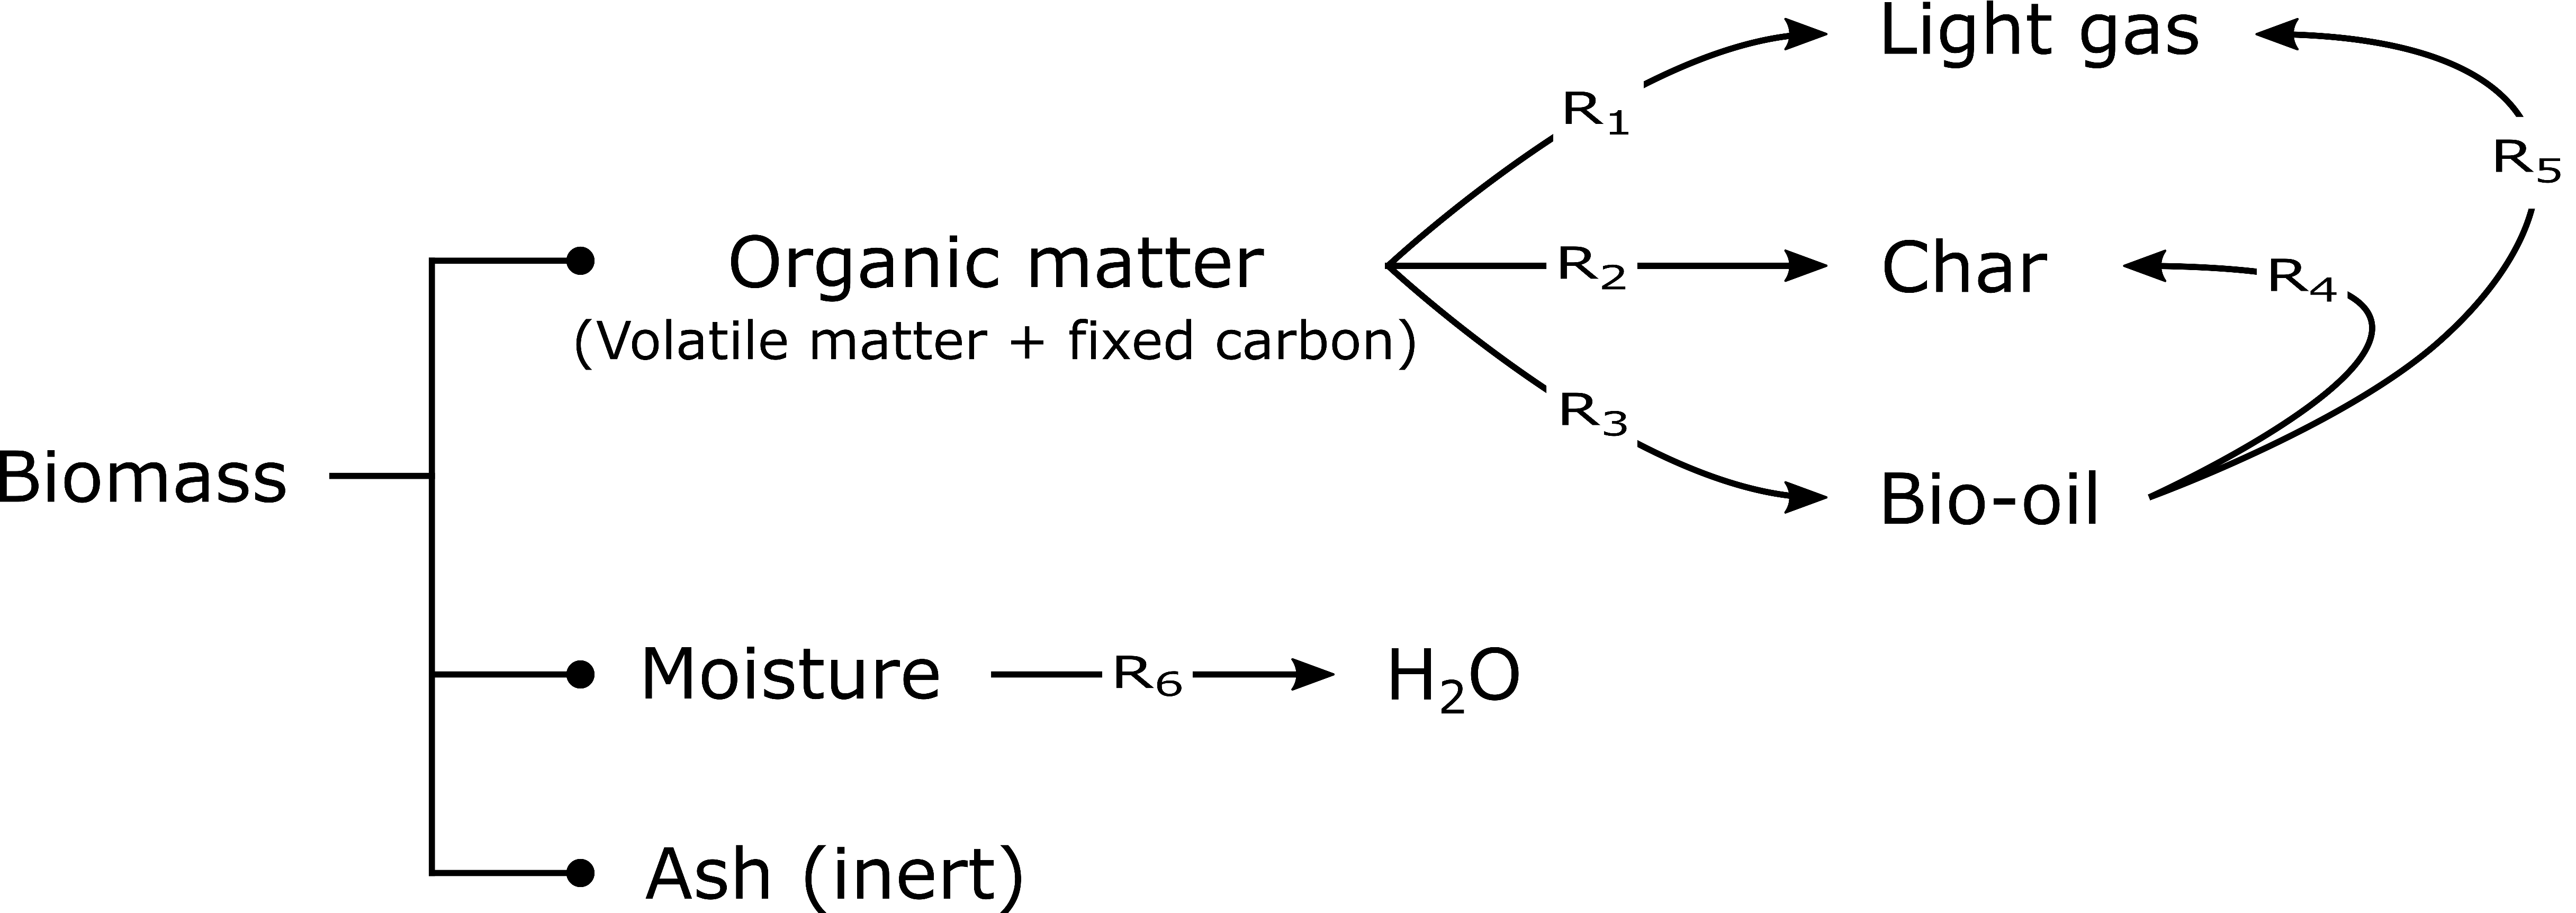
\includegraphics[width=1.0\textwidth]{kinetics.pdf}
    \caption{\textcolor{blue}{Diagram of the Di Blasi pyrolysis kinetics scheme for conversion of biomass to gas, bio-oil, and char products. Solid arrows depict primary pyrolysis reactions, dashed arrows depict bio-oil degradation reactions, and the dotted arrow depicts moisture vaporization.}}
    \label{fig:blasi}
\end{figure}

\noindent The pyrolysis reactions were modeled as first-order Arrhenius type equations where the reaction rate is given as

\begin{equation}
    r_i = C_i\,A_i\,e^{-E_i / R\,T}
\end{equation}

\noindent where r$_\text{i}$ is the rate of reaction i such that C$_\text{i}$ is a mass based concentration of the reactant species, A$_\text{i}$ is the pre-factor (1/s), E$_\text{i}$ is the activation energy (kJ/mol), R is the gas constant, and T is the reaction temperature (K). Kinetic parameters for each reaction are listed in Table \ref{tab:kinetic-params} where $\Delta$H is the heat of reaction (kJ/kg). Based on the work performed by Lu et al.\cite{lu2020bridging}, the Di Blasi kinetics overpredict light gas production when using a coarse-grained DEM model. Consequently, we modified the pre-factor parameter for reaction 4 by a factor of 0.2 which was determined by comparisons with NREL experiments \cite{French-2021}.

\begin{table}[H]
    \centering
    \caption{Kinetic parameters based on the Di Blasi biomass pyrolysis scheme where $\Delta$H$_\text{vap}$ is the heat of vaporization of water.}
    \begin{tabular}{clrrr}
        \toprule
        Reaction & A (1/s) & E (kJ/mol) & $\Delta$H (kJ/kg) & Reference \\
        \midrule
        1 & $4.38 \times 10^9$    & 152.7 & -20                    & \cite{Blasi-2001} \\
        2 & $3.75 \times 10^6$    & 111.7 & -20                    & \cite{Blasi-2001} \\
        3 & $1.08 \times 10^{10}$ & 148.0 & 255                    & \cite{Blasi-2001} \\
        4 & $8.56 \times 10^5$    & 108.0 & -42                    & \cite{Blasi-1993,lu2020bridging} \\
        5 & $1.00 \times 10^6$    & 108.0 & -42                    & \cite{Blasi-1993} \\
        6 & $5.13 \times 10^6$    & 87.6  & $\Delta$H$_\text{vap}$ & \cite{Chan-1985} \\
        \bottomrule
    \end{tabular}
    \label{tab:kinetic-params}
\end{table}

\noindent The char resulting from the pyrolysis reactions participate in surface reaction wih gas phas chemical species, including char--H$_2$O, char--CO$_2$, and char--H$_2$ reactions. The char surface reaction model assumes the reactions follows the unreacted-core shrinking model \cite{Chyou-2013}, accounting for diffusion effects on the char reaction rates. The kinetics paramters for the three char surface reactions (char--H$_2$O, char--CO$_2$, and char--H$_2$) were obtained from Wen and Chaung \cite{Wen1979entr}.

\subsection{CFD-DEM simulation}

A coarse-grained CFD-DEM model was implemented for biomass pyrolysis in MFiX, an open-source, Fortran-based code \cite{Syamlal-1993}. The coarse-grained CFD-DEM model used in this work is an extension of the standard MFiX release. Gas phase transport was described using conservation equations of mass, momentum, energy, and chemical species in the Eulerian framework (Equations \ref{eq:gas-trans-mass}--\ref{eq:gas-trans-chemical}, respectively).

\begin{align}
    \frac{d(\epsilon_g \rho_g)}{dt} + \nabla (\epsilon_g \rho_g u_g) &= S_\rho \label{eq:gas-trans-mass} \\
    \frac{d(\epsilon_g \rho_g u_g)}{dt} + \nabla (\epsilon_g \rho_g u_g u_g) &= -\epsilon_g \nabla p + \nabla (\epsilon_g \tau) + \epsilon_g \rho_g g + S_u \\
    \frac{d(\epsilon_g \rho_g E)}{dt} + \nabla (\epsilon_g \rho_g u_g E) &= -\nabla Q + S_E \\
    \frac{d(\epsilon_g \rho_g Y_i)}{dt} + \nabla (\epsilon_g \rho_g u_g Y_i) &= -\nabla (D_i \nabla Y_i) + S_{Y_i} \label{eq:gas-trans-chemical}
\end{align}

\noindent where $\epsilon_\text{g}$, $\rho_\text{g}$, u$_\text{g}$, p, $\tau$, Q, and Y$_\text{i}$ are gas phase volume fraction, density, velocity, pressure, stress tensor, conductive heat flux, and ith chemical species, respectively; while t is time, g is acceleration due to gravity, D$_\text{i}$ is mass diffusion coefficient for species, S$_\rho$, S$_\text{u}$, S$_\text{E}$, and S$_\text{Yi}$ are mass, momentum, energy, and chemical species source terms, respectively.

Fixed quantities of discrete particles with identical initial conditions were lumped into a computational coarse-grained parcel (CGP), whose motion was governed by Newton’s second law of motion. All particle forces and contact dynamics were calculated on the parcel scale, whereas heat and mass transfers were calculated on particle scale and projected to the entire parcel. Accordingly, all particles in same coarse-grained parcel possess identical temperature, chemical species concentration, and momentum. The mass and diameter of each coarse-grained parcel is such that

\begin{align}
    m_{CGP} &= m_p W \\
    d_{CGP} &= d_p W^{1/3}
\end{align}

\noindent where m$_\text{CGP}$ is CGP mass, m$_\text{p}$ is distinct particle mass, W parcel statistical weight, d$_\text{CGP}$ is CGP diameter, and d$_\text{p}$ is distinct particle diameter. Instantaneous accelerations (translational and rotational) for each coarse-grained parcel were calculated as

\begin{align}
    \frac{d u_{CGP}}{dt} &= g - \frac{F_p}{m_{CGP}} + \frac{F_c}{m_{CGP}} + \frac{F_d}{m_{CGP}} \\
    \frac{d \omega_{CGP}}{dt} &= \frac{T_{CGP}}{I_{CGP}}
\end{align}

\noindent where u$_\text{CGP}$ and $\omega_\text{CGP}$ are the CGP translational and rotational velocities, g is acceleration due to gravity, m$_\text{CGP}$ is CGP mass, T$_\text{CGP}$ is net torque on the CGP, and I$_\text{CGP}$ is CGP moment of inertia. The term F$_\text{p}$ represents pressure gradient force and was calculated as a product of the CGP volume and pressure gradient. The CGP collision forces F$_\text{C}$ (parcel-parcel and parcel-wall collisions) were modeled according to the linear spring-dashpot model \cite{Navarro-2013}. Since the number of CGP collisions is significantly lower than the number of collisions expected in a system with distinct particles, the CGP coefficient of restitution was modified as a correction for energy dissipations during collisions. The proposed modification to the CGP coefficient of restitution made use of the kinetic theory of granular flow \cite{Lu-2014} as

\begin{equation}
    e_{CGP} = \sqrt{1 + (e_p^2 - 1) W^{1/3}}
\end{equation}

\noindent where e$_\text{CGP}$ is CGP coefficient of restitution and e$_\text{p}$ is distinct particle coefficient of restitution.

Two different drag models were used to estimate CGP drag force F$_\text{d}$ based on well-documented difference in the fluidization behavior of sand and biomass in the literature \cite{Oliveira-2013}. Drag force was estimated using the Ganser-corrected Gidaspow drag model for sand particles (bed material) and a filtered drag model for biomass particles. The Ganser correction \cite{Ganser-1993} was coupled to the Gidaspow model \cite{Gidaspow-1994} to account for non-sphericity of the sand particles as expressed below.

\begin{equation}
    \beta_{Ganser} =
    \begin{cases}
        \beta_{Ergun} & \text{if } \epsilon_g \leq 0.8 \\
        \beta_{WenYu} & \text{if } \epsilon_g > 0.8
    \end{cases}
\end{equation}

\begin{align}
    \beta_{Ergun} &= 150 \frac{(1 - \epsilon_g)^2 \mu_g}{\epsilon_g d^2_{CGP} \phi^2} + 1.75 \frac{(1 - \epsilon_g) \rho_g}{\epsilon_g d_{CGP} \phi} |u_g - u_{CGP}| \\
    \beta_{WenYu} &= \frac{3}{4} C_d \frac{(1 - \epsilon_g) \rho_g}{d_{CGP} \phi} |u_g - u_{CGP}| \epsilon_g^{-2.65}
\end{align}

\begin{equation}
    C_d =
    \begin{cases}
        \frac{24}{Re K_1} (1 + 0.1118(Re K_1 K_2)^{0.6567}) + \frac{0.4305 K_2}{1 + \frac{3305}{Re K_1 K_2}} & \text{if } Re < 1,000 \\
        0.44 & \text{if } Re \geq 1,000 \\
        0.0 & \text{if } Re = 0.0
    \end{cases}
\end{equation}

\begin{align}
    K_1 &= \left(\frac{1}{3} + \frac{2}{3} \phi^{-0.5} \right)^{-1} - 2.25 \frac{d_{CGP}}{D} \\
    K_2 &= 10^{1.8148 (-log \phi)^{0.5743}}
\end{align}

The filtered drag model (modified Sarkar drag model) used in this work for biomass particles was proposed by Gao et al. \cite{Gao-2018} and was found by the authors to have relatively high prediction strength across multiple flow regimes in a fluidized bed. The modified Sarkar drag model was derived from a fine-grid simulation using the Wen-Yu drag model and can be computed as follows:

\begin{equation}
    \beta_{Sarkar} = \beta_{WenYu} (1 - H_{Sakar})
\end{equation}

\begin{equation}
    H_{Sakar} =
    \begin{cases}
        0.95 \left(1 - e^{-\alpha_1 \alpha_2 (u_{\text{slip}}^* - u_0)^p} \right) & u_{\text{slip}}^* > u_0 \\
        0.0 & u_{\text{slip}}^* \leq u_0
    \end{cases}
\end{equation}

\begin{equation}
    u_{\text{slip}}^* = \frac{|u_g - u_{CGP}|}{u_t}
\end{equation}

\begin{align}
    \alpha_1 &= \frac{\left(a_1 + a_2(1 - \epsilon_g) + a_3(1 - \epsilon_g)^2 + a_4(1 - \epsilon_g)^3 + a_5(1 - \epsilon_g)^4 \right)}{1 + e^{100 \left((1 - \epsilon_g) - 0.55 \right)}} \\
    \alpha_2 &= \left(1 + \frac{a_6}{\Delta_{\text{filter}}^*} + \frac{a_7}{(\Delta_{\text{filter}}^*)^2} \right) \left(1 + \frac{a_8}{(u_{\text{slip}}^*)^2} \right)
\end{align}

\begin{equation}
    u_0 = \frac{a_9 + a_{10} (1 - \epsilon_g)}{0.01 + (1 - \epsilon_g)^{a_{11}}} \left(1 + \frac{a_{12}}{\Delta_{\text{filter}}^*} + \frac{a_{13}}{(\Delta_{\text{filter}}^*)^2} \right)
\end{equation}

\begin{equation}
    p = \left(a_{14} + a_{15}(1 - \epsilon_g) + a_{16}(1 - \epsilon_g)^2 \right) \left(1 + \frac{a_{17}}{\Delta_{\text{filter}}^*} + \frac{a_{18}}{(\Delta_{\text{filter}}^*)^2} \right)
\end{equation}

\begin{align}
    \Delta_{\text{filter}}^* &= max\left( \frac{g \Delta_{\text{filter}}}{u_t^2}, \; \frac{1}{2} \right) \\
    \Delta_{\text{filter}} &= 2 (\Delta_x \times \Delta_y \times \Delta_z)^{1/3}
\end{align}

\begin{equation}
    u_t = \frac{g d_{CGP}^2 (\rho_{CGP} - \rho_g)}{18 \mu_g}
\end{equation}

\begin{equation}
    \begin{matrix}
        a_1    & a_2    & a_3 \\
        a_4    & a_5    & a_6 \\
        a_7    & a_8    & a_9 \\
        a_{10} & a_{11} & a_{12} \\
        a_{13} & a_{14} & a_{15} \\
        a_{16} & a_{17} & a_{18} \\
    \end{matrix}
    \; =
    \begin{array}{rrr}
        0.75597773   & 2.73931487  & -5.60196497 \\
        -1.65853820  & 16.70299223 & -0.44145335 \\
        0.18195034   & -0.01827347 & 0.28441799  \\
        -1.943573770 & 0.22177961  & 0.31175890  \\
        -0.15971960  & 0.47750002  & 0.062794180 \\
        5.13011673   & 0.67680355  & -0.54535726 \\
    \end{array}
\end{equation}

% Model parameters
% ----------------------------------------------------------------------------

\section{Model parameters}

Particle size distribution of the biomass feedstock along with the mass flow rate associated with each size bin is given in Table \ref{tab:params-part-size}. The initial biomass chemical composition used for the Di Blasi kinetics model is shown in Table \ref{tab:params-chem-biomass}. Other parameters related to the biomass and sand particles along with reactor operation and simulation settings are provided in Table \ref{tab:params}. Biomass particle characteristics and properties are representative of loblolly pine while the bed particle characteristics are for a typical sand material. Operating conditions and reactor dimensions are based on the previously discussed NREL 2FBR fluidized bed pyrolysis unit.

\begin{table}[H]
    \centering
    \caption{Particle size distribution for the biomass feedstock.}
    \label{tab:params-part-size}
    \begin{tabular}{>{\centering}p{2.5cm} >{\raggedleft}p{2.2cm} >{\raggedleft\arraybackslash}p{2.5cm}}
        \toprule
        Sauter mean diameter (\textmugreek m) & Mass fraction (\%) & Mass flow rate (kg/hr) \\
        \midrule
        278 & 34.3 & 0.051 \\
        344 & 50.7 & 0.076 \\
        426 & 12.0 & 0.018 \\
        \bottomrule
    \end{tabular}
\end{table}

\begin{table}[H]
    \centering
    \caption{Initial chemical composition of the biomass feedstock for the Di Blasi kinetics model.}
    \label{tab:params-chem-biomass}
    \begin{tabular}{lrr}
        \toprule
        Species & Mass fraction (\%) & Density (kg/m$^3$) \\
        \midrule
        moisture & 4.0  & 1,000 \\
        wood     & 95.9 & 550 \\
        ash      & 0.1  & 2,000 \\
        char     & 0.0  & 300 \\
        \bottomrule
    \end{tabular}
\end{table}

\begin{table}[H]
    \centering
    \caption{Parameters for the biomass, sand (bed material), and reactor operation. Biomass C$_\text{p}$ calculated from particle composition. Parameters for simulation settings also given.}
    \label{tab:params}
    \begin{tabular}{lll}
        \toprule
        Parameter & Value & Description \\
        \midrule
        biomass particle \\
        e$_\text{p}$    & 0.2        & particle-particle coefficient of restitution \\
        e$_\text{w}$    & 0.2        & particle-wall coefficient of restitution \\
        e$_\text{s}$    & 0.2        & particle-sand coefficient of restitution \\
        $\mu_\text{p}$  & 0.1        & particle-particle coefficient of friction \\
        $\mu_\text{w}$  & 0.2        & particle-wall coefficient of friction \\
        $\mu_\text{s}$  & 0.1        & particle-sand coefficient of friction \\
        k$_\text{n}$    & 100 N/m    & particle spring constant \\
        \\
        sand particle \\
        d$_\text{p}$       & 453 $\mu$m          & particle diameter \\
        $\rho_\text{p}$    & 2500 kg/m$^3$       & particle density \\
        C$_\text{p}$       & 830 J/(kg\,K)      & particle heat capacity \\
        $\phi$             & 0.94                & particle sphericity \\
        e$_\text{p}$       & 0.61                & particle-particle coefficient of restitution \\
        e$_\text{w}$       & 0.61                & particle-wall coefficient of restitution \\
        $\mu_\text{p}$     & 0.1                 & particle-particle coefficient of friction \\
        $\mu_\text{w}$     & 0.2                 & particle-wall coefficient of friction \\
        k$_\text{n}$       & 100 N/m             & particle spring constant \\
        \\
        reactor operation \\
        d$_\text{inner}$      & 5.25 cm       & inner reactor diameter \\
        H$_\text{reactor}$    & 43.18 cm      & reactor height \\
        H$_\text{static}$     & 10.16 cm      & static bed height \\
        p$_\text{gas}$        & 101.325 kPa   & gas pressure \\
        T$_\text{gas}$        & 773.15 K      & gas temperature \\
        Q$_\text{gas}$        & 14 SLM        & inlet gas flowrate \\
        \\
        simulation settings \\
        $\Delta_\text{x} \times \Delta_\text{y} \times \Delta_\text{z}$ & $2.0 \times 2.0 \times 2.0$ mm & CFD cell size \\
        $\Delta_\text{x}$   & varies & time step \\
        wt$_\text{bio}$      & 5     & biomass parcel statistical weight \\
        wt$_\text{sand}$     & 20     & sand parcel statistical weight \\
        s$_\text{gas}$               & ideal  & gas phase equation of state \\
        \bottomrule
    \end{tabular}
\end{table}

Table \ref{tab:flowrates} summarizes the CFD simulations conducted for this study. Each row represents a different simulation case that was performed for a particular gas composition. An additional $2.83\times10^{-5}$ m$^3$/s of N$_2$ at 500$^\circ$C was supplied at the fluidizing gas inlet and $2.55\times10^{-5}$ m$^3$/s of N$_2$ at 25$^\circ$C was supplied at the biomass feed inlet for all cases. For cases 1--7, the total flow rate was kept constant, resulting in a constant superficial gas velocity inside the reactor. For cases 8--12, the gas flow rates were modified to maintain a constant fluidization number (U$_\text{s}$/U$_\text{mf}$) of 3 in each simulation. Also, cases 8--12 represent H$_2$ mass fractions of 0.2, 0.4, 0.6, 0.8 and 1. Pure hydrogen is modeled because of its drastically different properties compared to the other gases (see following section); however, its applicability in experiments is limited due to safety concerns.

% I updated the flowrate used for N2 in Case 1 and Case 8 to exclude the constant 2.83e-5 m3/s flowrate of N2 since the remaining entries did not include this portion of the flow and it was confusing

\begin{table}[H]
    \centering
    \caption{CFD--DEM simulation cases for the different gas mixtures.}
    \begin{tabular}{lllccccc}
        \toprule
           &               & U$_\text{s}$ (m/s)  &\multicolumn{5}{c}{Mass fraction (--)}  \\
        ID & Gas mixture   & at 500$^\circ$C     & N$_2$ & H$_2$ & CO  & CO$_2$ & CH$_4$  \\
        \midrule
        1  & N$_2$         & $6.61\times10^{-4}$ & 1.0   & 0.0   & 0.0 & 0.0    & 0.0     \\
        2  & H$_2$         & $6.61\times10^{-4}$ & 0.0   & 1.0   & 0.0 & 0.0    & 0.0     \\
        3  & CO            & $6.61\times10^{-4}$ & 0.0   & 0.0   & 1.0 & 0.0    & 0.0     \\
        4  & CO$_2$        & $6.61\times10^{-4}$ & 0.0   & 0.0   & 0.0 & 1.0    & 0.0     \\
        5  & CH$_4$        & $6.61\times10^{-4}$ & 0.0   & 0.0   & 0.0 & 0.0    & 1.0     \\
        6  & N$_2$/CO      & $6.61\times10^{-4}$ & 0.5   & 0.0   & 0.5 & 0.0    & 0.0     \\
        7  & N$_2$/CO$_2$  & $6.61\times10^{-4}$ & 0.5   & 0.0   & 0.0 & 0.5    & 0.0     \\
        8  & N$_2$/H$_2$   & $8.65\times10^{-4}$ & 0.8   & 0.2   & 0.0 & 0.0    & 0.0     \\
        9  & N$_2$/H$_2$   & $1.02\times10^{-3}$ & 0.6   & 0.4   & 0.0 & 0.0    & 0.0     \\
        10 & N$_2$/H$_2$   & $1.15\times10^{-3}$ & 0.4   & 0.6   & 0.0 & 0.0    & 0.0     \\
        11 & N$_2$/H$_2$   & $1.24\times10^{-3}$ & 0.2   & 0.8   & 0.0 & 0.0    & 0.0     \\
        12 & H$_2$         & $1.32\times10^{-3}$ & 0.0   & 1.0   & 0.0 & 0.0    & 0.0     \\
        \bottomrule
    \end{tabular}
    \label{tab:flowrates}
\end{table}

% Results and discussion
% ----------------------------------------------------------------------------

\section{Results and discussion}

This section provides results and related discussions for modeling the effects of different fluidization gases on the operation of a bubbling fluidized bed reactor. Gas effects on the pyrolysis yields of the biomass feedstock are also presented and discussed.

\subsection{Gas mixture properties}

Comparisons of the calculated viscosity of a H$_2$/N$_2$ gas mixture to measured values obtained from literature are shown in Figure \ref{fig:gas-mu-h2n2-validate}. The models by Herning and Zipperer as well as Brokaw match well with the experimental data for a range of mixture ratios. This is contradictory to the Davidson report which does not recommend the Herning and Zipperer model for hydrogen mixtures \cite{Davidson-1993}. The Davidson and Graham models significantly underpredict the mixture viscosity while the Wilke model tends to overestimate the viscosity. Similar results are obtained for a H$_2$/O$_2$ gas mixture as shown in Figure \ref{fig:gas-mu-h2o2-validate}.

\begin{figure}[H]
    \centering
    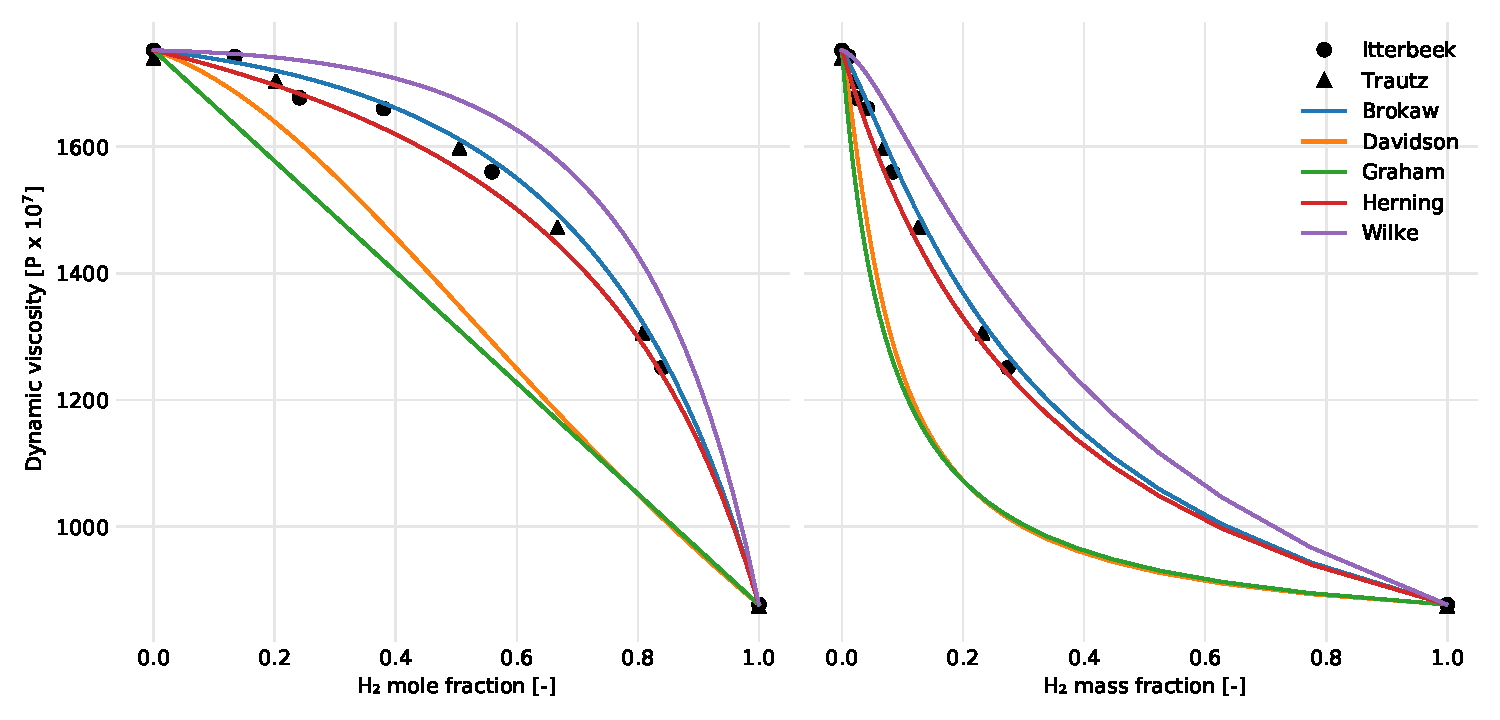
\includegraphics[width=\textwidth]{figures/gas-mu-h2n2-validate.pdf}
    \caption{Viscosity of a H$_2$/N$_2$ mixture at 291.1 K (18$^\circ$C). Calculated values represented by line profiles. Experiment data points from \cite{Itterbeek-1947,Trautz-1929} shown as symbols.}
    \label{fig:gas-mu-h2n2-validate}
\end{figure}

\begin{figure}[H]
    \centering
    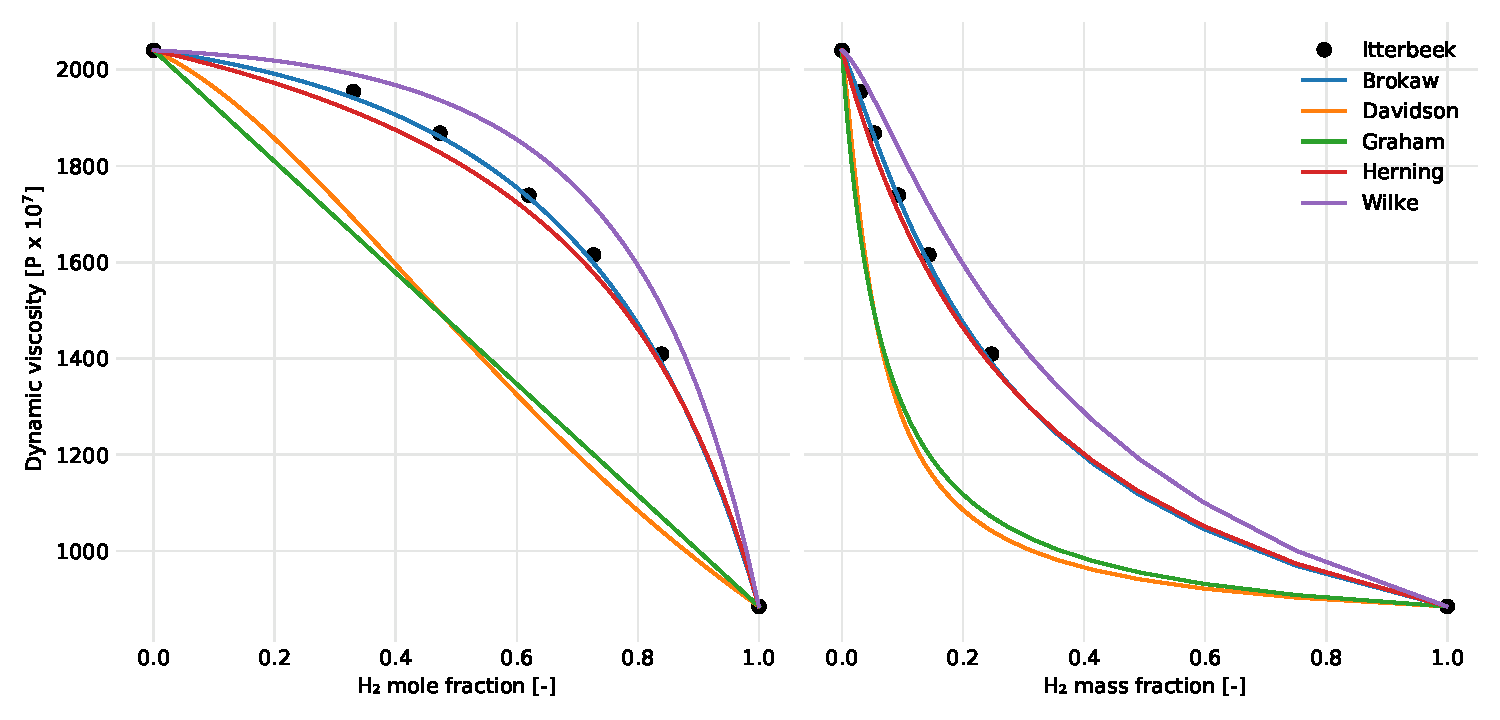
\includegraphics[width=\textwidth]{figures/gas-mu-h2o2-validate.pdf}
    \caption{Viscosity of a H$_2$/O$_2$ mixture at 293.6 K (20$^\circ$C). Calculated values represented by line profiles. Experiment data points from \cite{Itterbeek-1947} shown as symbols.}
    \label{fig:gas-mu-h2o2-validate}
\end{figure}

Properties for molecular weight, viscosity, and density for the gas mixtures investigated in this paper are shown in Figure \ref{fig:mix-properties}. Similar to the individual gas properties, the mixture properties were calculated at 101,325 Pa and 773.15 K (500$^\circ$C). The viscosity of the gas mixture was determined using the Herning and Zipperer method (Equation \ref{eq:herning}). The mole fraction of each gas in the mixture is given by the values shown at the top of each column in the figure. For example, the nitrogen and hydrogen mixture is comprised of 22\% nitrogen and 78\% hydrogen which is labeled as $0.22 + 0.78$. As expected, the carbon dioxide mixture is the heaviest in terms of molecular weight and density while the nitrogen and hydrogen mixture is the lightest. The most viscous mixture is the nitrogen and carbon monoxide where as the hydrogen mixtures are the least viscous.

\begin{figure}[H]
    \centering
    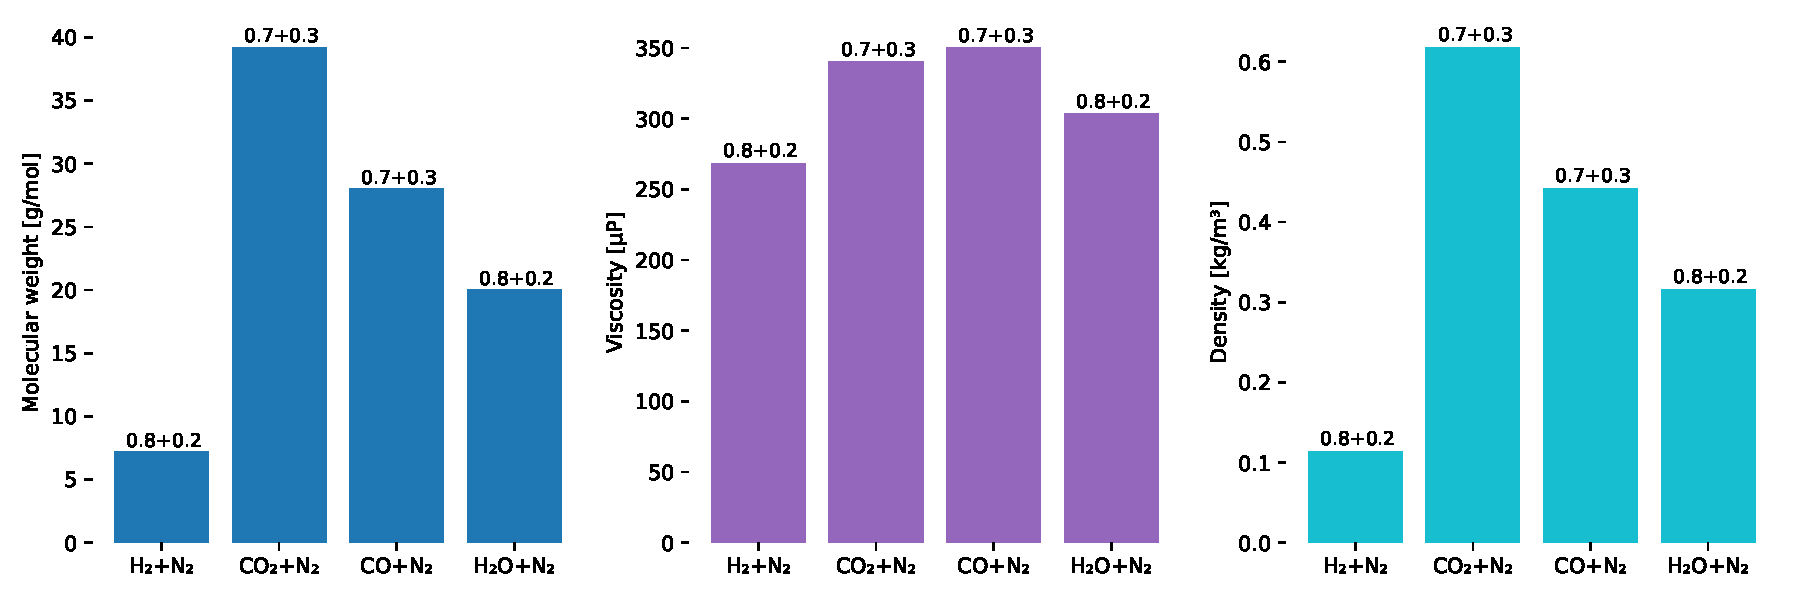
\includegraphics[width=\textwidth]{mix-properties.pdf}
    \caption{Comparison of gas mixture properties for molecular weight, viscosity, and density at 101,325 Pa and 773.15 K. Mole fraction of each gas component is shown at the top of each column.}
    \label{fig:mix-properties}
\end{figure}

\subsection{Fluidization characteristics}\label{sec:fluidization-charact}

Minimum fluidization velocity (U$_\text{mf}$) of the bed material for the different fluidization gases is presented in Table \ref{tab:umf-sand}. Hydrogen requires about twice the gas velocity to fluidize the bed of sand compared to the nitrogen, carbon monoxide, and carbon dioxide gases. This is due to hydrogen's lower viscosity and much lower density compared to the other gases. Water vapor and methane require moderately higher fluidization velocities compared to the nitrogen gas. A comparison of U$_\text{mf}$ for the various fluidization gases is displayed in Figure \ref{fig:umf-usumf-gases}.

\begin{table}[H]
    \centering
    \caption{Minimum fluidization velocity (m/s) of the bed material calculated from various correlations for different fluidization gases. Last row represents the average U$_\text{mf}$ value for each gas.}
    \label{tab:umf-sand}
    \begin{tabular}{lrrrrrr}
        \toprule
        U$_\text{mf}$ & N$_2$ & H$_2$ & H$_2$O & CO & CO$_2$ & CH$_4$ \\
        \midrule
        Ergun         & 0.14 & 0.30 & 0.18 & 0.15 & 0.16 & 0.23 \\
        Grace         & 0.10 & 0.21 & 0.13 & 0.11 & 0.11 & 0.16 \\
        Richardson    & 0.10 & 0.20 & 0.12 & 0.10 & 0.11 & 0.15 \\
        Wen and Yu    & 0.08 & 0.17 & 0.11 & 0.09 & 0.09 & 0.13 \\
        average       & 0.11 & 0.22 & 0.14 & 0.11 & 0.12 & 0.17 \\
        \bottomrule
    \end{tabular}
\end{table}

The superficial gas velocity (U$_\text{s}$) of the nitrogen gas flow is calculated as 0.3072 m/s which is based on the 14 SLM gas flow through the distributor plate. Using this value, the ratio of U$_\text{s}$ to U$_\text{mf}$ is shown in Table \ref{tab:us-umf-ratio} for different fluidization gases. The BFB pyrolysis reactor at NREL typically operates at a U$_\text{s}$/U$_\text{mf}$ of 3 with nitrogen gas. For gases such as H$_2$, H$_2$O, CO, CO$_2$, and CH$_4$, the gas flow into the reactor must be increased to have similar fluidized bed characteristics as the nitrogen case. A comparison of the increased U$_\text{s}$ for each gas along with the associated U$_\text{s}$/U$_\text{mf}$ is shown in Figure \ref{fig:us-usumf-gases}. As expected, the hydrogen gas flow must be approximately doubled compared to the nitrogen case to achieve similar fluidization of the bed material.

\begin{table}[H]
    \centering
    \caption{Ratio of U$_\text{s}$ to U$_\text{mf}$ for different fluidization gases. Last row represents the average U$_\text{s}$/U$_\text{mf}$ value for each gas.}
    \label{tab:us-umf-ratio}
    \begin{tabular}{lrrrrrr}
        \toprule
        U$_\text{s}$/U$_\text{mf}$ & N$_2$ & H$_2$ & H$_2$O & CO & CO$_2$ & CH$_4$ \\
        \midrule
        Ergun                      & 2.13 & 1.04 & 1.67 & 2.02 & 1.97 & 1.34 \\
        Grace                      & 2.99 & 1.47 & 2.35 & 2.84 & 2.76 & 1.88 \\
        Richardson                 & 3.16 & 1.55 & 2.48 & 3.00 & 2.91 & 1.98 \\
        Wen and Yu                 & 3.69 & 1.82 & 2.90 & 3.50 & 3.39 & 2.32 \\
        average                    & 2.99 & 1.47 & 2.35 & 2.84 & 2.76 & 1.88 \\
        \bottomrule
    \end{tabular}
\end{table}

\begin{figure}[H]
    \centering
    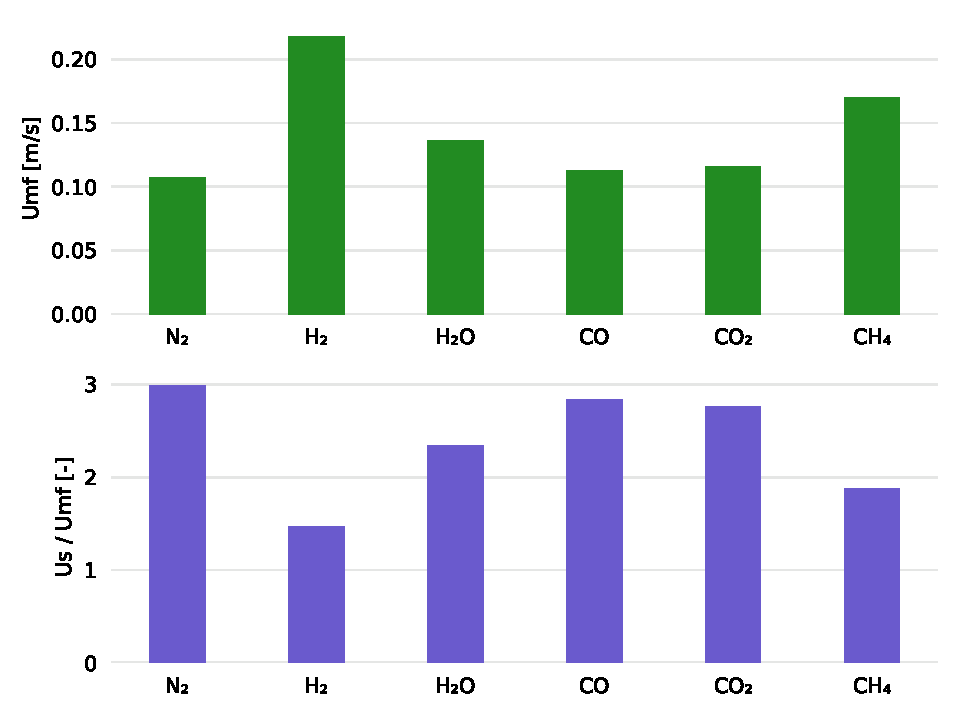
\includegraphics[width=0.8\textwidth]{figures/umf-usumf-gases.pdf}
    \caption{Comparison of the minimum fluidization velocity (U$_\text{mf}$) and the ratio of U$_\text{s}$/U$_\text{mf}$ for different fluidization gases. Superficial gas velocity is U$_\text{s}$.}
    \label{fig:umf-usumf-gases}
\end{figure}

\begin{figure}[H]
    \centering
    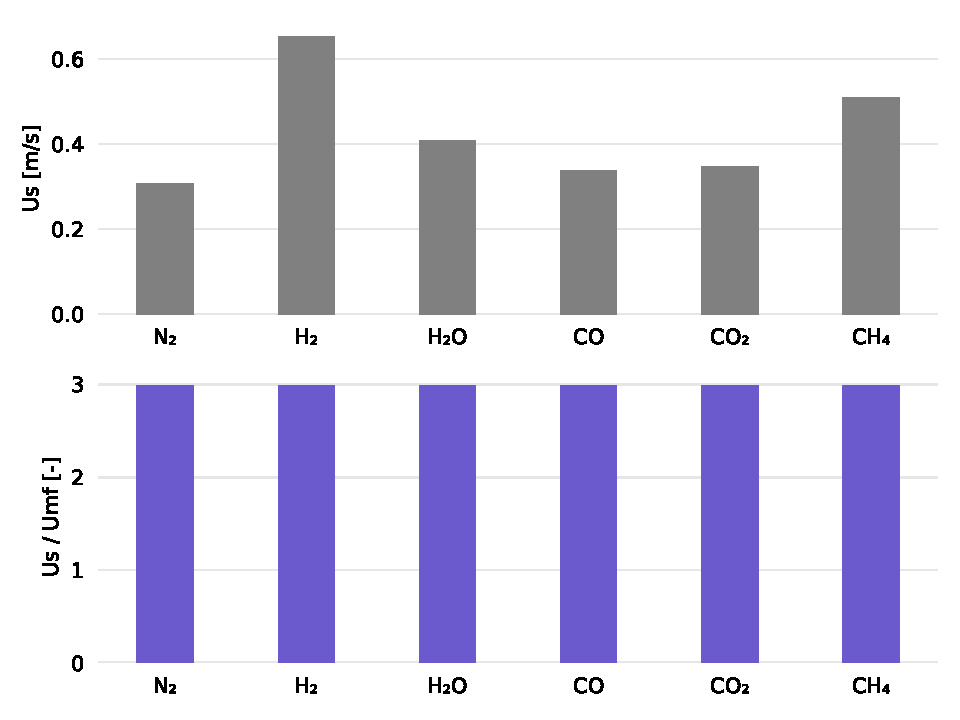
\includegraphics[width=0.8\textwidth]{figures/us-usumf-gases.pdf}
    \caption{Comparison of the superficial gas velocity (U$_\text{s}$) and the associated U$_\text{s}$/U$_\text{mf}$ for different fluidization gases. Minimum fluidization velocity is U$_\text{mf}$.}
    \label{fig:us-usumf-gases}
\end{figure}

The Reynolds number was calculated using an average biomass particle diameter of 369.4 $\mu$m and the mean U$_\text{mf}$ value. Next, the Nusselt number along with the associated convective heat transfer coefficient were calculated for each carrier gas as shown in Table \ref{tab:biomass-hconv} and Figure \ref{fig:biomass-hconv}. The highest heat transfer coefficient is estimated for H$_2$ while the second highest result is for CH$_4$. This is largely due to the higher thermal conductivity of the hydrogen and methane compared to the other gases. Due to the higher heat transfer rate to the biomass particle in the hydrogen environment, one can expect the biomass to pyrolyze more quickly with the hydrogen carrier gas.

\begin{table}[H]
    \centering
    \caption{Comparison of the Reynolds number, Nusselt number, and convective heat transfer coefficient (h) for different fluidization gases.}
    \label{tab:biomass-hconv}
    \begin{tabular}{lrrrr}
        \toprule
        Gas & U$_\text{mf}$ & Re & Nu & h \\
        \midrule
        N$_2$  & 0.11 & 0.48 & 2.55 & 369.45  \\
        H$_2$  & 0.22 & 0.14 & 2.26 & 2224.25 \\
        H$_2$O & 0.14 & 0.50 & 2.56 & 464.54  \\
        CO     & 0.11 & 0.53 & 2.58 & 389.53  \\
        CO$_2$ & 0.12 & 0.89 & 2.81 & 399.83  \\
        CH$_4$ & 0.17 & 0.70 & 2.69 & 862.61  \\
        \bottomrule
    \end{tabular}
\end{table}

\begin{figure}[H]
    \centering
    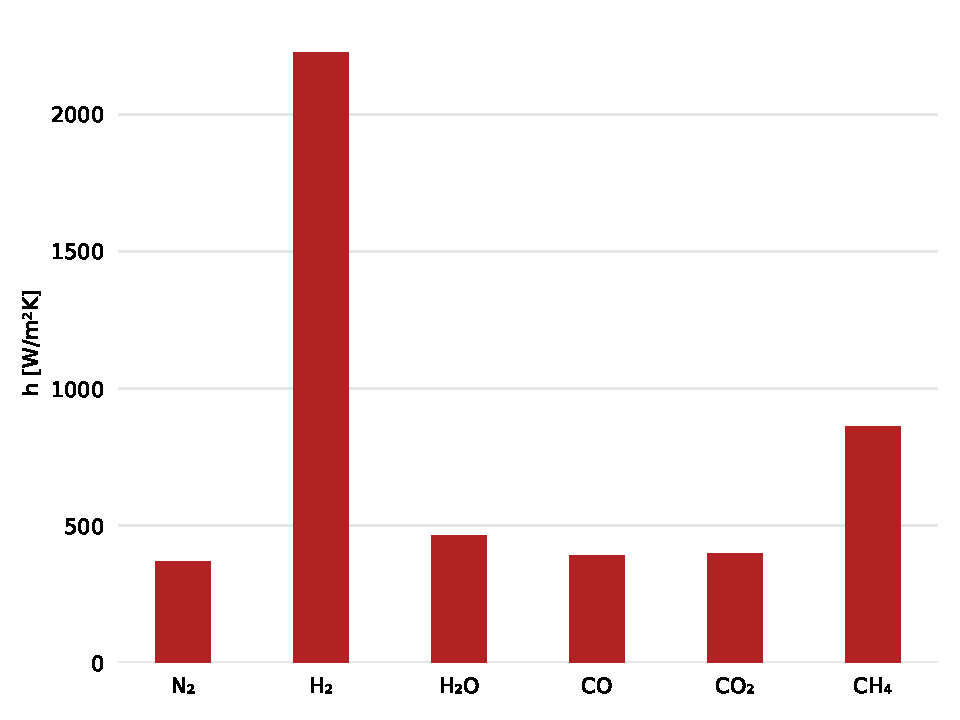
\includegraphics[width=0.8\textwidth]{figures/biomass_hconv.pdf}
    \caption{Convective heat transfer coefficient (h) for different fluidization gases. Values based on average biomass particle size and average minimum fluidization velocity.}
    \label{fig:biomass-hconv}
\end{figure}

\subsection{Limiting factors for biomass pyrolysis}

Gas influence on the pyrolysis limiting regimes is shown in Figure \ref{fig:biot-pyro-gases} for a biomass particle diameter of 369.4 $\mu$m. The regime map suggests that gas properties have little effect on the limiting mode of pyrolysis. However, when comparing a range of particle diameters, the differences are more pronounced as seen in Figure \ref{fig:biot-pyro-diams}. For larger particles, conduction becomes the limiting mode of pyrolysis especially for the hydrogen gas. For smaller particles, nitrogen gas promotes isothermal conditions along with a kinetically limited regime.

\begin{figure}[H]
    \centering
    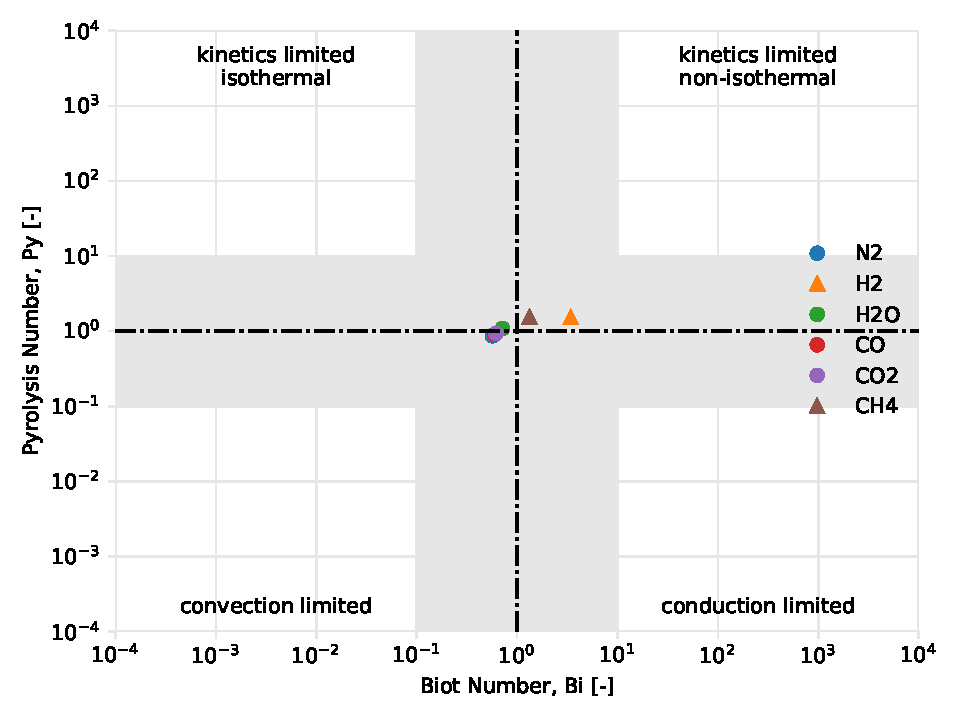
\includegraphics[width=0.8\textwidth]{figures/biot-pyro-gases.pdf}
    \caption{Comparison of carrier gas effects on pyrolysis regime for a 369.4 $\mu$m biomass particle. Grey region means no dominant mechanism controlling pyrolysis.}
    \label{fig:biot-pyro-gases}
\end{figure}

\begin{figure}[H]
    \centering
    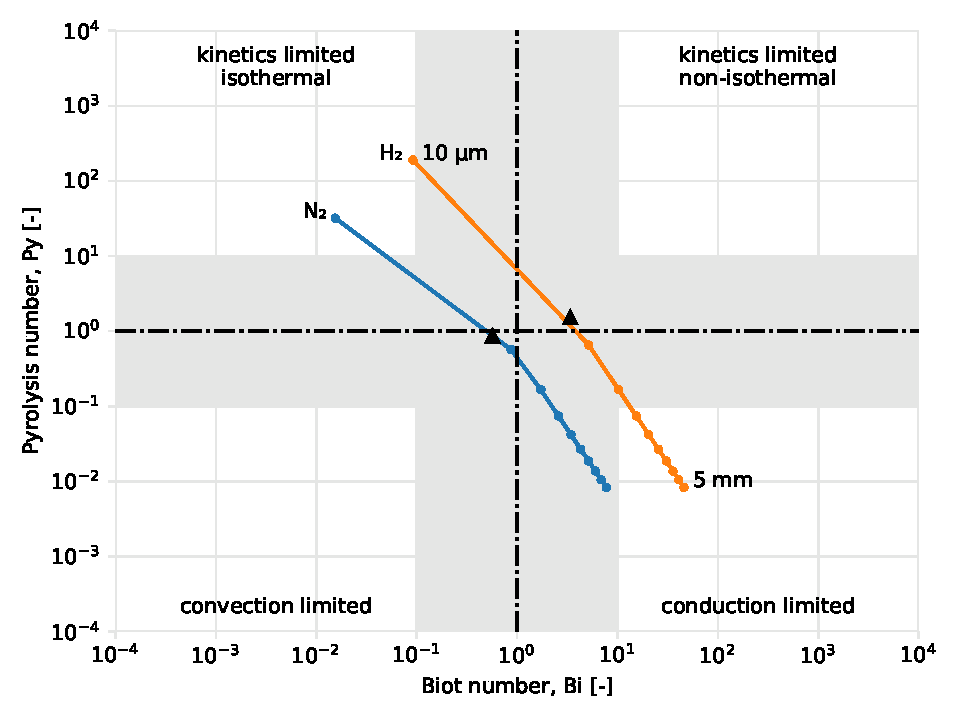
\includegraphics[width=0.8\textwidth]{figures/biot-pyro-diams.pdf}
    \caption{Comparison of nitrogen and hydrogen gas effects for biomass particles ranging from 10$\mu$m to 5 mm in diameter. Triangle markers symbolize 369.4 $\mu$m biomass particle diameter. Grey region means no dominant mechanism controlling pyrolysis.}
    \label{fig:biot-pyro-diams}
\end{figure}

\subsection{CFD-DEM validation}

The predicted yield of pyrolysis products (bio-oil, light gases, and biochar) was validated against experimental data of biomass pyrolysis using the same NREL 2FBR reactor system that was modeled and simulated in this work \cite{French-2021}. The process variables used in the experimental work are consistent with those implemented for the N$_2$ and H$_2$ cases (run ID = 1 and 2, respectively). The mass closure of the experimental data was about 94\%, therefore a mass proportional modification of the original data was performed to enforce 100\% mass closure and form a proper basis of comparison to the CFD--DEM simulation predictions. Table \ref{tab:cfddem-validation} shows that the predicted yields of pyrolysis products closely follow the experimental data. The magnitude of the relative prediction deviation ranged between 0.1\% and 9.0\%.

The prediction performance of the CFD--DEM model was highest for bio-oil, with a maximum absolute relative deviation of 1\%. The light gas yield for the N$_2$ case was overpredicted relative to the eperimental data, whereas the inverse was found for the H$_2$ case, where light gas was underpredicted. Similarly, biochar was slightly overpredicted for the H$_2$ but underpredicted for the N$_2$ case.

\begin{table}[H]
    \centering
    \caption{CFD–DEM model validation against experimental data. Product yields were calculated on a biomass weight basis. Experiment data from \cite{French-2021}.}
    \label{tab:cfddem-validation}
    \begin{tabular}{cccccc}
        \toprule
               & Fluidizing   & Pyrolysis & \multicolumn{2}{c}{Pyrolysis yield (wt.\%)} & Relative \\
        Run ID & gas          & product   & Experiment & Simulation                     & deviation (\%) \\
        \midrule
        1 & N$_2$ & bio-oil   & 74.5      & 74.5       & 0.1     \\
        1 & N$_2$ & light gas & 12.3      & 13.4       & 9.0     \\
        1 & N$_2$ & biochar   & 13.2      & 12.1       & --8.6   \\
        2 & H$_2$ & bio-oil   & 73.7      & 74,5       & 1.0     \\
        2 & H$_2$ & light gas & 15.0      & 13.8       & --7.8   \\
        2 & H$_2$ & biochar   & 11.3      & 11.7       & 3.6     \\
        \bottomrule
    \end{tabular}
\end{table}

% \subsection{Fluidizing gas effect on pyrolysis performance at a constant flow rate/velocity (U$_s$)}
\subsection{Fluidizing gas effect on pyrolysis performance at a constant flow rate/velocity (U\texorpdfstring{$_s$}{s})}

The yields of pyrolysis bio-oil, light gas, and biochar for the different fluidizing gases at a constant flow rate of 14 SLPM ($6.61\times10^{-4}$ m$^3$/s) are compared in Figure \ref{fig:cfd-product-yield}. The observed differences in the pyrolysis product distribution among the fluidizing gases were minimal. The highest bio-oil yield of 74.8 wt.\% and lowest bio-oil yield of 73.8 wt.\% were obtained when pure CH$_4$ and CO were used as fluidizing gas, respectively. The bio-oil yield was slightly higher when any of H$_2$, CH$_4$, and CO$_2$ replaced N$_2$ as the fluidizing gas. The evidence reviewed here suggests that light gas may be recirculated at a constant flow rate during pyrolysis without causing substantial losses in bio-oil yield.

\begin{figure}[H]
    \centering
    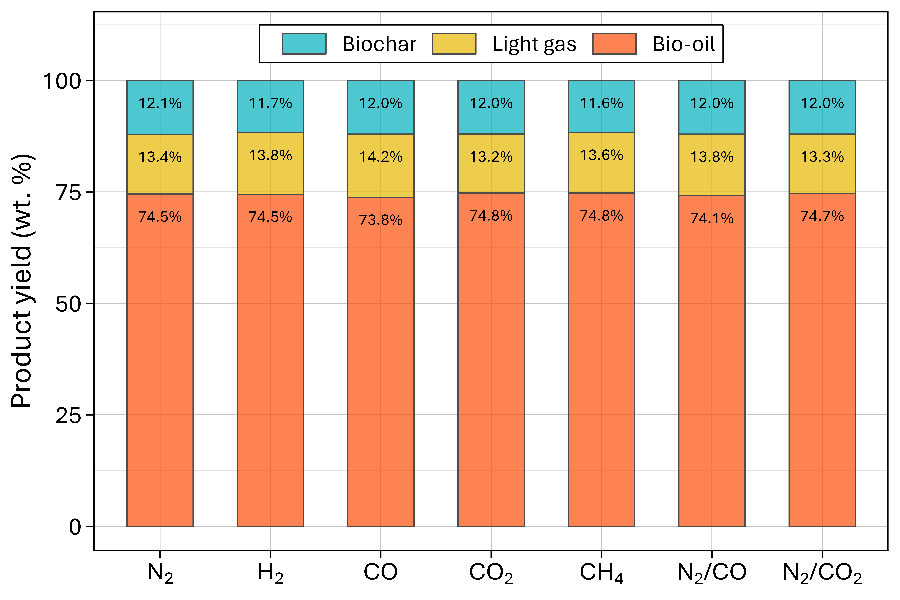
\includegraphics[width=1.0\textwidth]{figures/cfd-product-yield.pdf}
    \caption{Pyrolysis product distributions for different fluidizing gas at a constant flow rate. Product yields were calculated on a biomass weight basis.}
    \label{fig:cfd-product-yield}
\end{figure}

A summary of the particle residence time for each fluidizing gas considered is given in Table \ref{tab:particle-restime}. It was unsurprising to find that the median particle residence time increased with increasing initial diameter of the biomass particles. The difference in particle residence time among the fluidizing gases also generally increased with increasing initial diameter of biomass particles. In other words, the impact of fluidizing gas on particle residence time is stronger for larger particles and weaker for smaller particles.

\begin{table}[H]
    \centering
    \caption{Particle residence time of biomass particle for different fluidizing gas at a constant flow rate and different initial particle diameter where d$_p$ is initial biomass particle diameter.}
    \label{tab:particle-restime}
    \begin{tabular}{cccccc}
        \toprule
               & Fluidizing & \multicolumn{4}{c}{Median particle residence time (s)} \\
        Run ID & gas        & d$_p$ = 296 $\mu m$ & d$_p$ = 333 $\mu m$ & d$_p$ = 371 $\mu m$ & d$_p$ = 408 $\mu m$ \\
        \midrule
        1 & N$_2$        & 6.8 & 8.7  & 11.1  & 14.3 \\
        2 & H$_2$        & 9.5 & 14.4 & 18.4 & 21.1 \\
        3 & CO           & 6.9 & 8.9  & 11.0  & 14.1 \\
        4 & CO$_2$       & 6.3 & 7.9  & 10.5  & 12.5 \\
        5 & CH$_4$       & 7.3 & 10.5  & 14.1 & 18.1 \\
        6 & N$_2$/CO     & 6.8 & 9.0  & 12.2  & 14.3 \\
        7 & N$_2$/CO$_2$ & 6.5 & 8.2  & 10.0  & 12.9 \\
        \bottomrule
    \end{tabular}
\end{table}

Figure \ref{fig:cfd-temp-void-biooil} shows the gas phase temperature and void volume fraction profile along the reactor height for different fluidizing gas at a constant flow rate. The gas-phase temperature was higher in the freeboard than in the bed. This is attributed to the fact that enthalpy for biomass pyrolysis reactions is drawn from inside the bed because pyrolysis reactions occur predominantly inside the bed. Additionally, the gas temperature was relatively unchanged along the reactor height within the bed whereas, in the freeboard, the gas temperature increased towards the reactor outlet. Also noteworthy is the fact that the gas temperature along the reactor height was consistently highest when H$_2$ was used as fluidizing gas (Figure \ref{fig:cfd-temp-void-biooil}a). This observation is attributable to the large difference in the thermal conductivity of H$_2$ compared to the other fluidization gases (Figure \ref{fig:gas-properties}). It should be noted that the difference observed in the fluid temperature was less than 10$^{\circ}$C. The average height of the fluidized bed was about 0.14 m for all the fluidizing gases considered, except for H$_2$ and CH$_4$ which produced a lower bed height (Figure \ref{fig:cfd-temp-void-biooil}b). The bed height was determined as the position along the reactor height where the void volume fraction approached 0.7.

\begin{figure}[H]
    \centering
    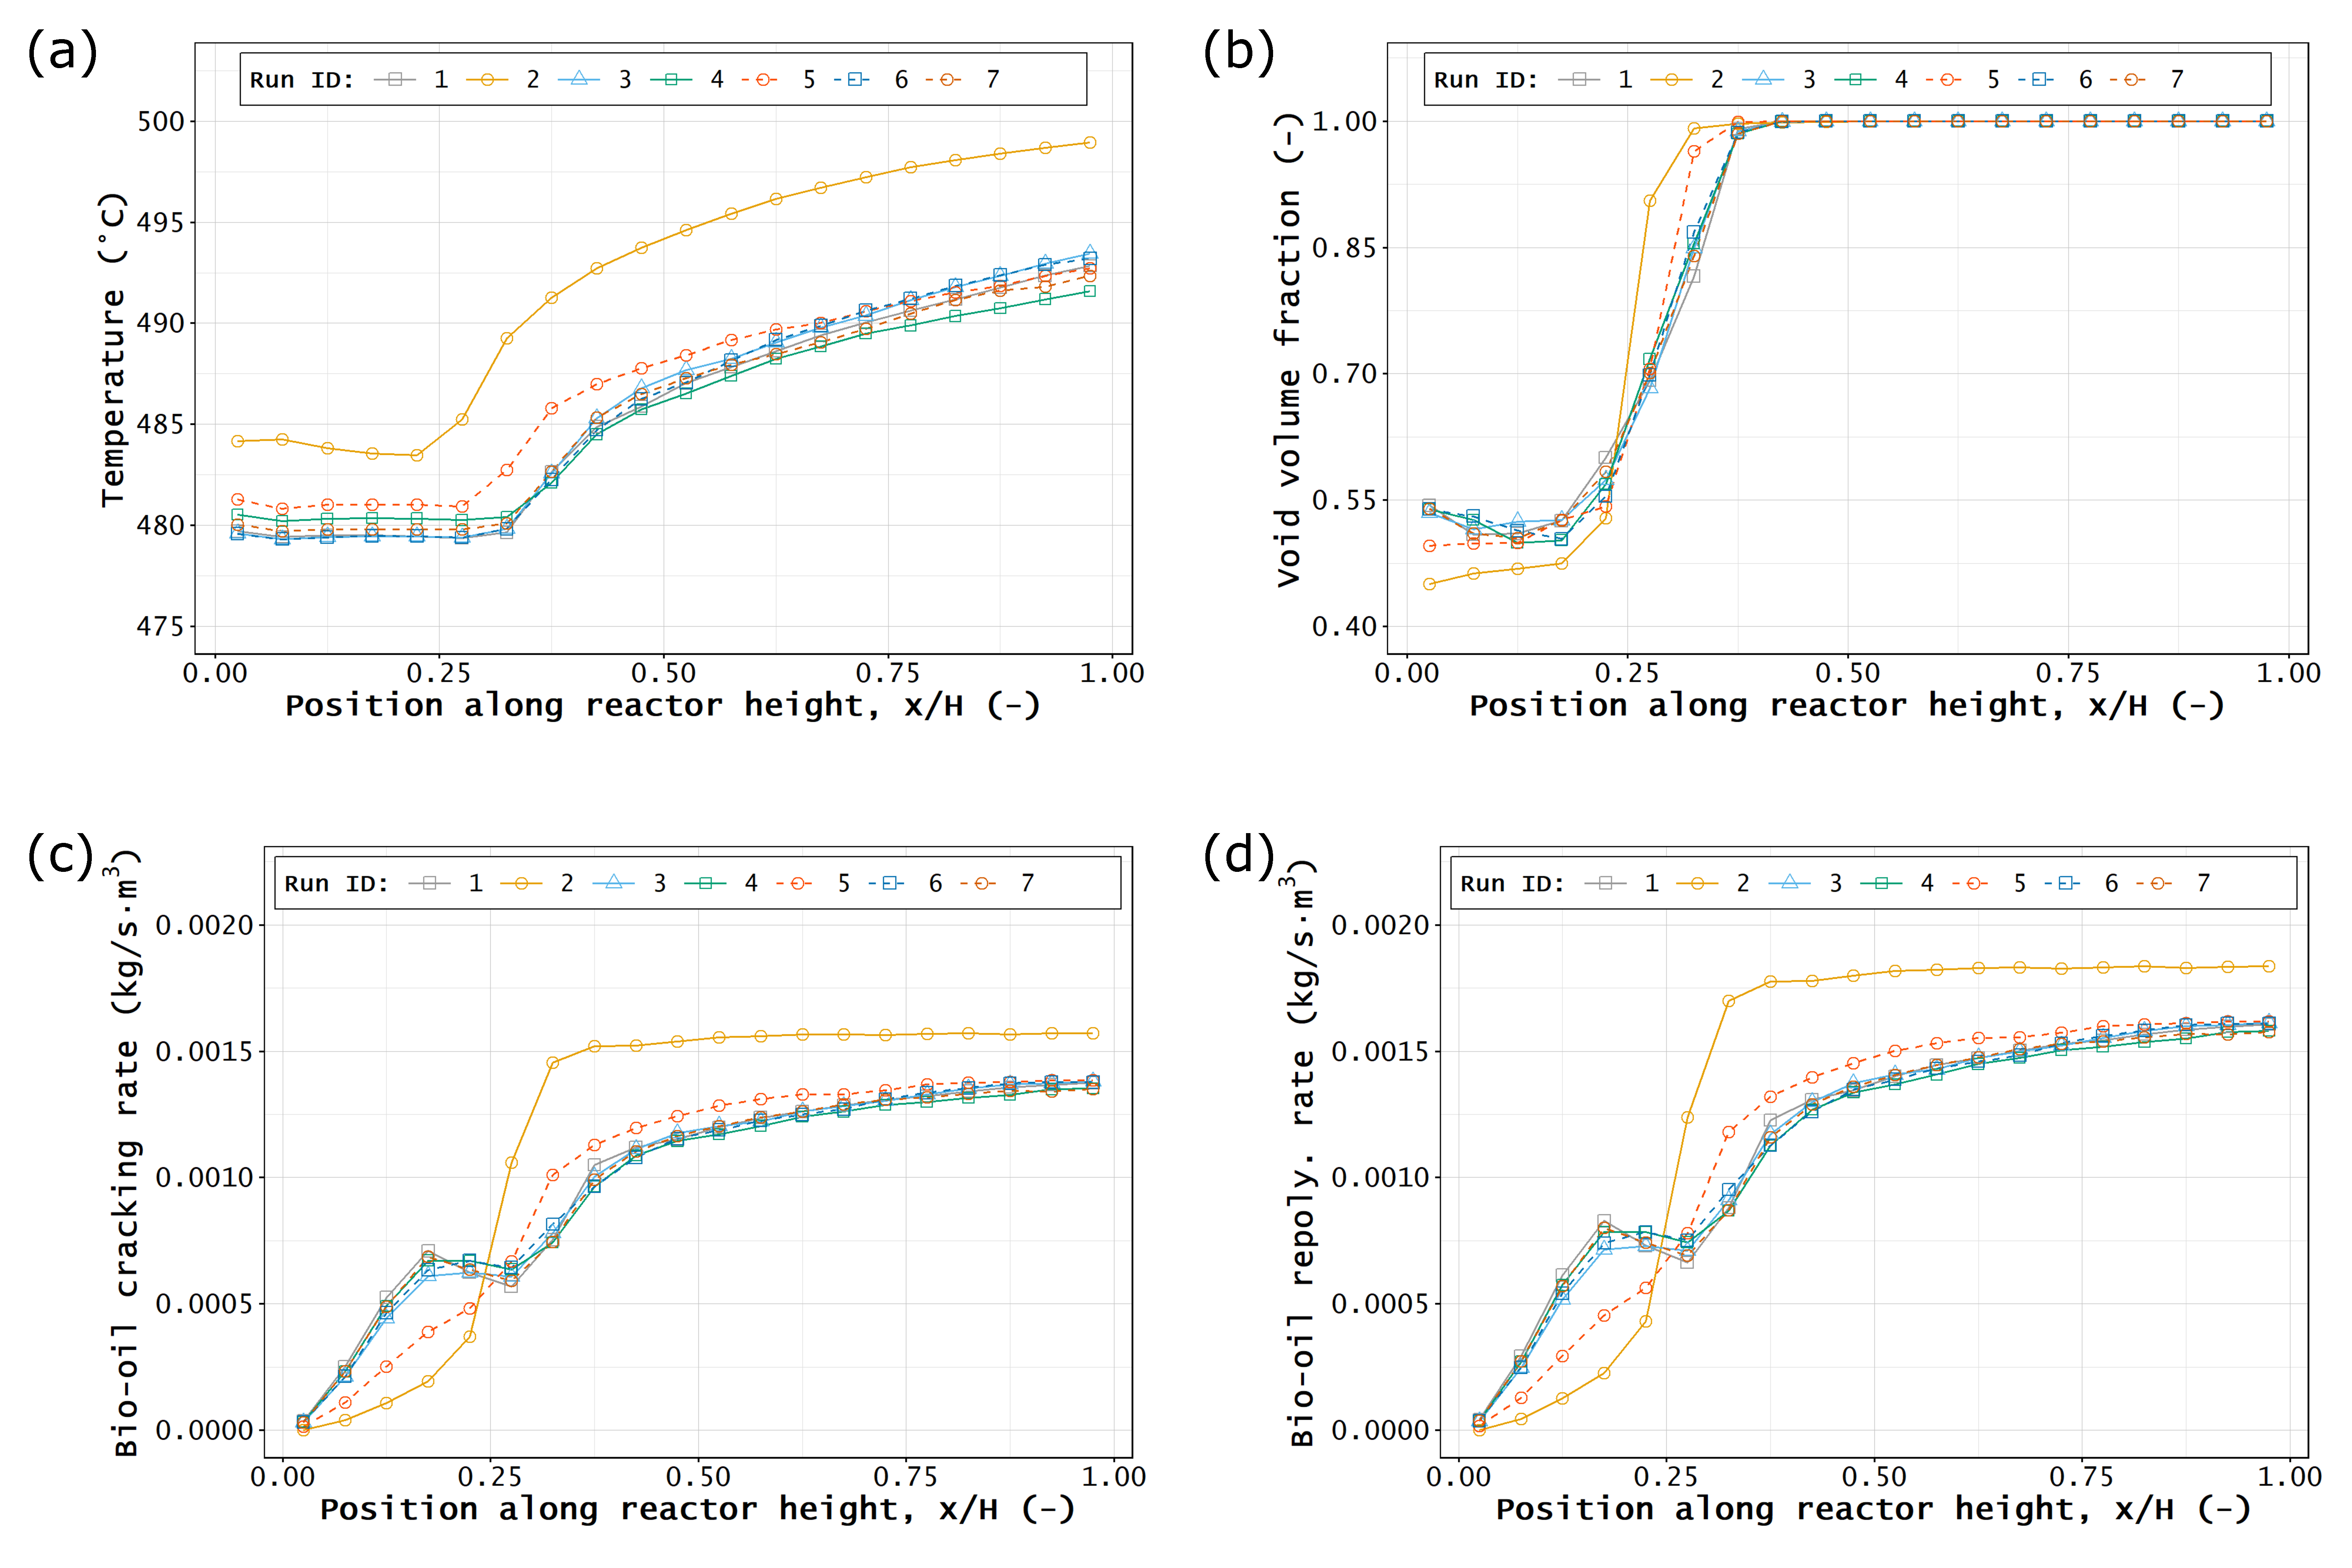
\includegraphics[width=1.0\textwidth]{figures/cfd-temp-void-biooil.pdf}
    \caption{Profile of (a) fluid temperature and (b) fluid volume fraction along the reactor height for different fluidizing gas at a constant flow rate. The reactor height (0.43 m) is denoted by the letter H.}
    \label{fig:cfd-temp-void-biooil}
\end{figure}

Char surface reactions were negligible under the pyrolysis conditions explored in this study. Notably, char--CO$_2$ and char--H$_2$O surface reaction rates were approximately six and three orders of magnitude lower than the primary biomass pyrolysis reactions, as depicted in Figure \ref{fig:heterogeneous-profiles}. Figure \ref{fig:heterogeneous-profiles} also illustrates the prevailing heterogeneous reaction profiles, underscoring the dominant influence of pyrolysis reactions within the reactor bed. Simultaneously, Figure \ref{fig:homogeneous-profiles} highlights the paramount role of homogeneous gas phase reactions in the freeboard region. These observations underscore the critical significance of pyrolysis reactions in the bed and emphasize the heightened importance of homogeneous gas phase reactions in the freeboard of the reactor. Furthermore, the impact of the fluidizing gas on the pyrolysis reaction rate profile was determined to be largely small. As anticipated, the concentration of CO$_2$ and CO species significantly influences the char--CO$_2$ and char--H$_2$O reaction rates, respectively. However, these reaction rates are several orders of magnitude lower than the pyrolysis reactions, rendering them negligible. Figure \ref{fig:homogeneous-profiles} also provides insights into the impact of each fluidizing gas on the homogeneous gas phase reaction profile. For instance, bio-oil cracking and repolymerization reactions (Figure \ref{fig:homogeneous-profiles} a and b) were most pronounced when H$_2$ was used as the fluidizing gas, aligning with the elevated temperature associated with H$_2$ fluidizing gas.

\begin{figure}[H]
    \centering
    \includegraphics[width=\textwidth]{heterogeneous-profiles.pdf}
    \caption{Heterogeneous reaction rate profiles inside the reactor as affected by different fluidizing gas at a constant velocity. (a) Biomass pyrolysis reaction rate profile, (b) Biomass tarring reaction rate profile, (c) Char--CO$_2$ surface reaction rate profile, and (d) Char--H$_2$O surface reaction rate profile. The reactor height (0.43 m) is denoted by the letter H.}
    \label{fig:heterogeneous-profiles}
\end{figure}

\begin{figure}[H]
    \centering
    \includegraphics[width=\textwidth]{homogeneous-profiles.pdf}
    \caption{Homogeneous reaction rate profiles inside the reactor as affected by different fluidizing gas at a constant velocity. (a) Bio-oil cracking reaction rate profile, (b) Bio-oil repolymerization reaction rate profile, (c) CH$_4$ steam reforming reaction rate profile, (d) Forward water gas shift (WGS) reaction rate profile, and (e) Reverse water gas shift reaction rate profile. The reactor height (0.43 m) is denoted by the letter H.}
    \label{fig:homogeneous-profiles}
\end{figure}

The observed degradation rates for both the particle and vapor phases were substantially affected by the fluidizing gas used. The shape of the bio-oil cracking rate profile along the reactor height was similar to that of the bio-oil repolymerization rate for all the fluidizing gases considered (Figure \ref{fig:cfd-temp-void-biooil}c and Figure \ref{fig:cfd-temp-void-biooil}d). Bio-oil degradation rates were higher in the freeboard than in the bed. The overall bio-oil degradation rates with H$_2$ as the fluidizing gas were substantially higher than those observed with other fluidizing gases. The reactor volume-averaged bio-oil cracking and repolymerization rates were $1.31\times10^{-3}$ and $1.54\times10^{-3}$ kg/s·m$^3$ for H$_2$, respectively $1.21\times10^{-3}$ and $1.42\times10^{-3}$ kg/s·m$^3$ for N$_2$, respectively. This data demonstrates that bio-oil degradation rates were 8\% higher when H$_2$ replaced N$_2$ as the fluidizing gas. This observation explains the reason why despite H$_2$ yielding the highest particle heating and mass-loss rates (Figure \ref{fig:cfd-masspercent}), and one of the longest residence times (Table \ref{tab:particle-restime}), its bio-oil yield is marginally different from the bio-oil yield with other fluidizing gases, especially N$_2$. When H$_2$ was used as fluidizing gas, biomass particles experienced significantly higher heating rates, and consequently higher mass-loss rates, compared to when other fluidizing gases were used. The impact of fluidizing gas on the heating and mass-loss rates was higher for larger particles. Generally, biomass heating and mass-loss rates follow the order: H$_2$ $>$ CH$_4$ $>$ CO $>$ N$_2$ $>$ N$_2$/CO $>$ N$_2$/CO$_2$ $>$ CO$_2$ which correlates well with the effective thermal conductivity of the fluidizing gas.

\begin{figure}[H]
    \centering
    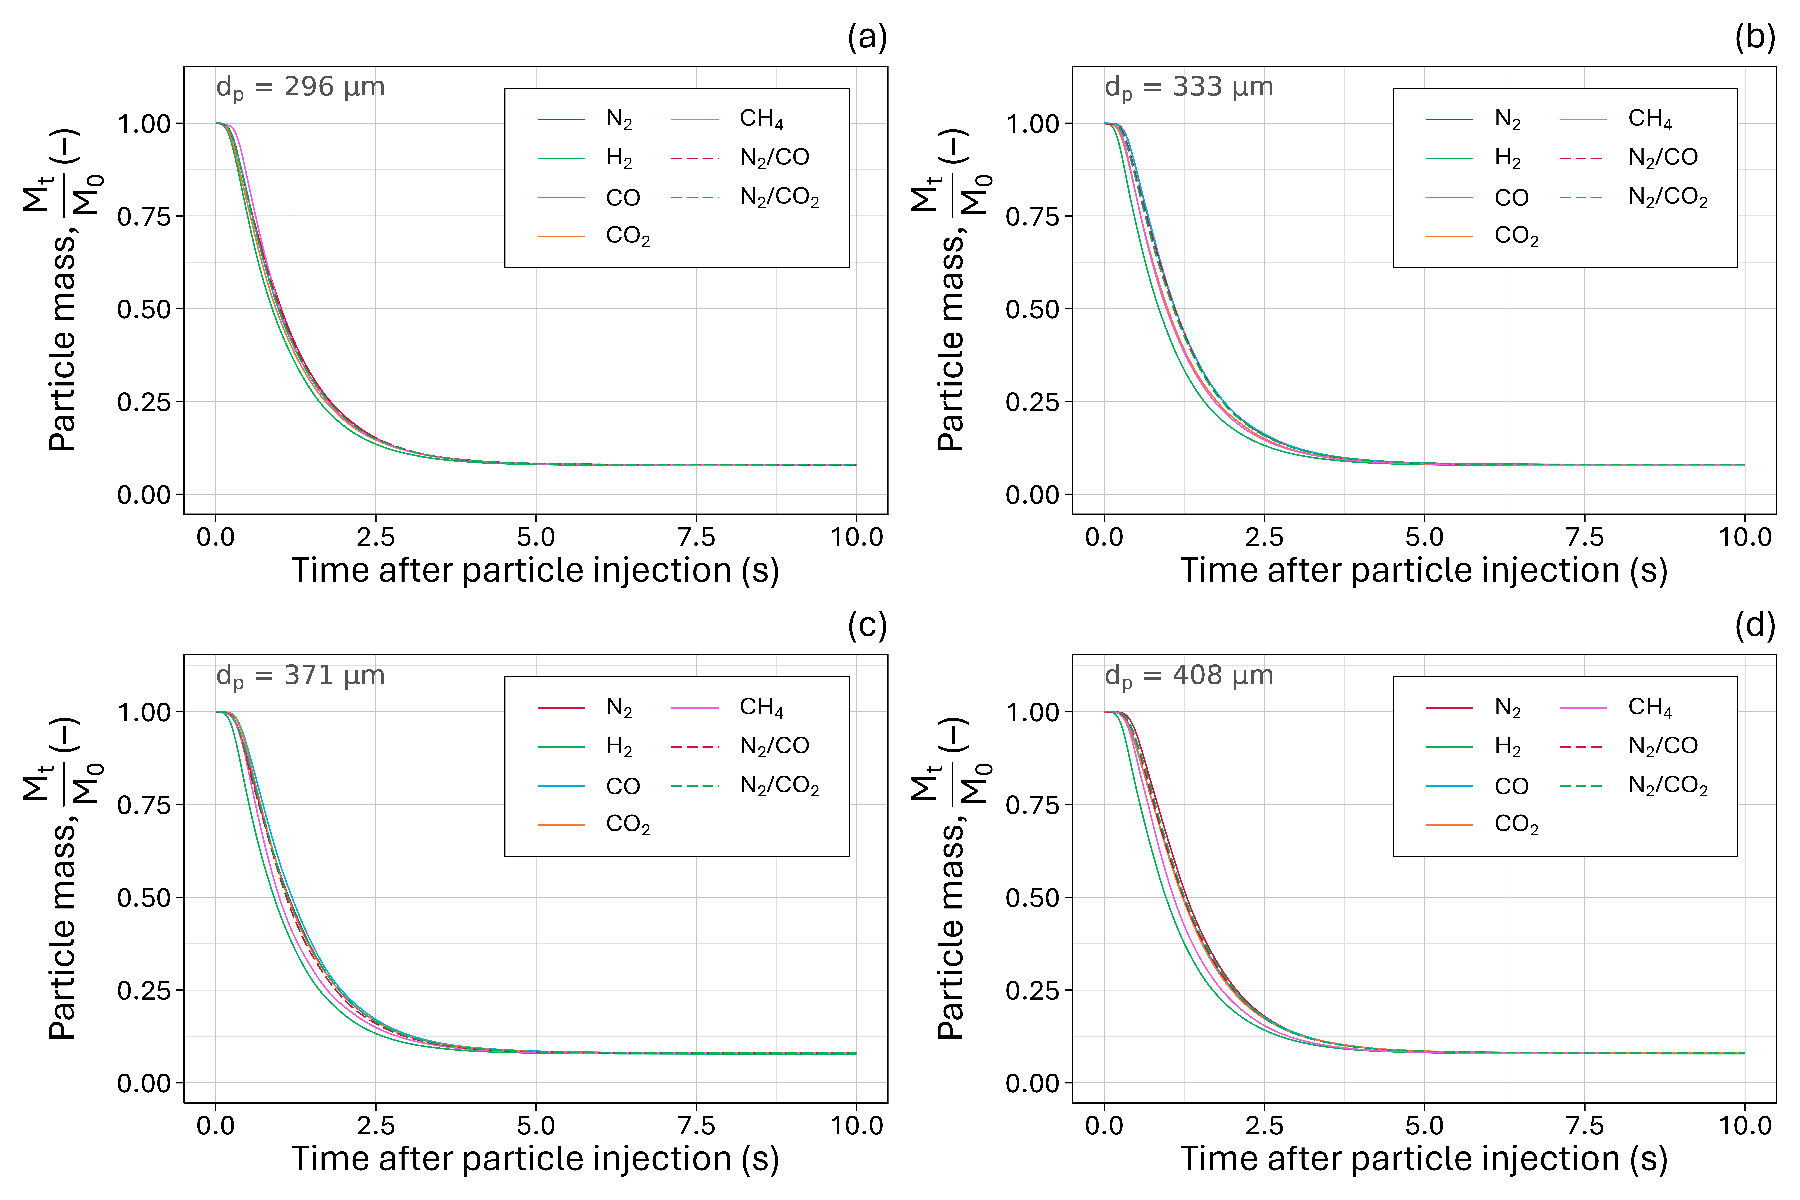
\includegraphics[width=1.0\textwidth]{figures/cfd-masspercent.pdf}
    \caption{Average biomass particle thermogravimetry curve for different fluidizing gas at a constant flow rate (a) nominal particle size = 296 $\mu m$, (b) nominal particle size = 333 $\mu m$, (c) nominal particle size = 371 $\mu m$, and (d) nominal particle size = 408 $\mu m$.}
    \label{fig:cfd-masspercent}
\end{figure}

Overall, the model results indicate that light gas produced during pyrolysis can be recirculated as fluidizing gas at a constant flow rate without detrimental consequences on pyrolysis performance. Additionally, we demonstrated that fluidizing gas can notably increase biomass heating and mass-loss rates (pyrolysis conversion rate). This suggests potential process intensification implications because heating and mass-loss rates represent a major bottleneck in conventional pyrolysis systems. Achieving increased heating and mass-loss rates may lead to significant improvement in process throughput and scaleup.

\subsection{Fluidizing gas effect on pyrolysis performance with constant fluidization number (\texorpdfstring{U$_\text{s}$/U$_\text{mf}$}{Us/Umf})}

As discussed in Section \ref{sec:fluidization-charact}, the value of U$_\text{s}$/U$_\text{mf}$ varies for each fluidizing gas composition when the flowrate is kept constant. As a result, the dynamic behavior of the bed, which U$_\text{s}$/U$_\text{mf}$ characterizes, varies with the gas composition. These differences are most pronounced between N$_2$ and H$_2$ which have U$_\text{s}$/U$_\text{mf}$ values of ~3.0 and ~1.5, respectively, when U$_\text{s}$ remains constant. To investigate the effect of gas properties on pyrolysis yields, the mass fraction of H$_2$ was varied between 0 and 1 (with the N$_2$ as the remaining fraction) while maintaining a constant U$_\text{s}$/U$_\text{mf}$ = 3.0. Figure \ref{fig:cfd-constuumf-particle-temp-density} shows the average particle temperature and mass as a function of time after injection into the reactor for each particle size in both N$_{2}$ and H$_{2}$ fluidizing gas streams. Here it can be seen, as for the constant $U_\text{s}$ case, the larger heat transfer coefficient associated with the H$_2$ fluidizing gas (h$_{\text{H}_2}$ = 2224.3, h$_{\text{N}_2}$ = 368.5 W/m$^2$K) result in greater rates of heat transfer and mass loss. Additionally, the nearly identical time distributions of the particle temperature and mass for H$_2$ with constant U$_\text{s}$ and U$_\text{s}$/U$_\text{mf}$ indicates that total heat transfer to a particle in bubbling fluidized bed is independent of the gas velocity. This is consistent with previous results that while convection increases with gas velocity, this increase is offset by decreases in conduction between solids in the bed \cite{Collier-2004,zhou2009particle}.

\begin{figure}[H]
    \centering
    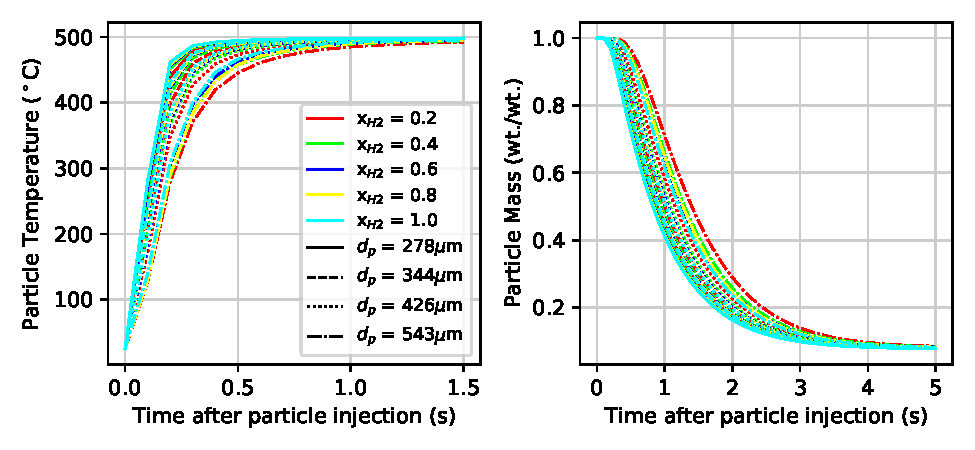
\includegraphics[width=\textwidth]{figures/cfd-constuumf-particle-temp-density.pdf}
    \caption{Average particle temperature (left) and density (right) as a function of residence time in reactor for N$_2$ and H$_2$ carrier gasses. For H$_2$ carrier gas, results with both constant U$_\text{s}$ and U$_\text{s}$/U$_\text{mf}$ are provided.}
    \label{fig:cfd-constuumf-particle-temp-density}
\end{figure}

At the reactor conditions and particle sizes investigated, the gas velocities are insufficient for biomass particles to elutriate from the reactor at their initial density and diameter. Therefore, the particle remains in the reactor until its size and mass are sufficiently reduced by pyrolysis to be ejected from the reactor. This can be seen in Figure \ref{fig:cfd-constuumf-terminal-vel}, which contains the particle diameter and density at which the terminal velocity, U$_\text{t}$, is equal to the gas velocity for each H$_2$ mass fraction investigated. At the initial particle density, the maximum diameter at which U$_\text{s}$ $\ge$ U$_\text{t}$ falls well outside of the initial paticle distribution in all cases. As as result, the particles remain in the reactor, losing size and mass as biomass is converted to bio-oil and char until their their terminal velocity is sufficiently small for elutriation to occur. As discussed previously, the lower density of H$_2$ reduces the drag induced on the particles by the flow. As a result the, switching the working fluid from N$_2$ to H$_2$ results in a significant decrease in the maximum particle size at which U$_\text{s}$ = U$_\text{t}$ for a given particle density (348 and 345 $\mu$m for Y$_{\text{H}_2}$ = 0 and 156 and 214 $\mu$m for Y$_{\text{H}_2}$ = 1 at the initial and char densities, respectively). When the gas velocity is increased to maintain constant U$_\text{s}$/U$_\text{mf}$, the increased gas velocity offsets the effect of the lower density, resulting in smaller decreases in the maximum particle diameter at which U$_\text{t}$ = U$_\text{s}$ for a given density. Specifically, the maximum diameters differ by 20 $\mu$m at the initial density and 30 $\mu$m across range of H$_2$ mass fractions. This produces a similar effect on the similar particle residence times, which can be seen in Figure \ref{fig:cfd-constuumf-rtd}, which contains the average residence time for each particle diameter plotted against the H$_2$ mass fraction in the fluidizing gas. Here, we see that while the particle residence time increases with increasing mass fraction of H$_2$, this effect is more pronounced when U$_\text{s}$ is held constant. This is particularly true for the largest particle sizes with the average residence time increasing 19\% between Y$_{\text{H}_2}$ = 0 and Y$_{\text{H}_2}$ = 1 for constant U$_\text{s}$/U$_\text{mf}$ and 45\% for constant U$_\text{s}$.

\begin{figure}[H]
    \centering
    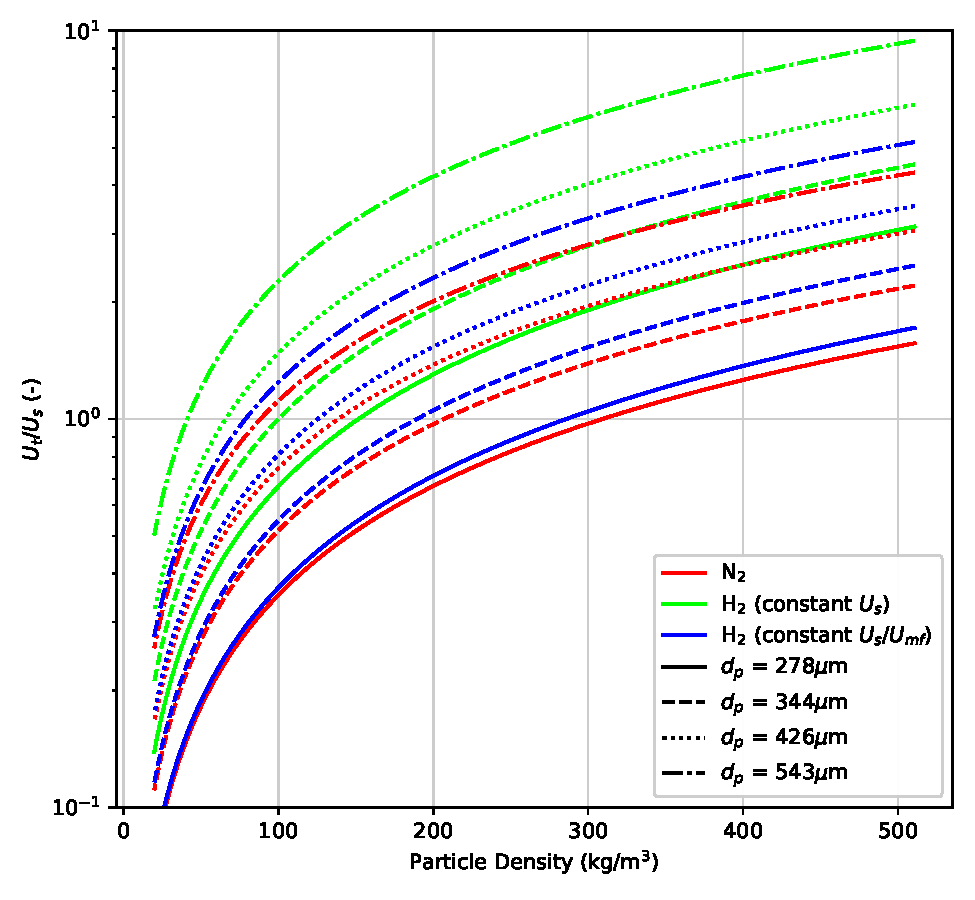
\includegraphics[width=0.8\textwidth]{figures/cfd-constuumf-terminal-vel.pdf}
    \caption{Particle diameter and density at which terminal velocity, U$_\text{t}$ is equal to the superficial gas velocity, U$_\text{s}$, for N$_2$ and H$_2$ carrier gasses. For H$_2$ carrier gas, results with both constant U$_\text{s}$ and U$_\text{s}$/U$_\text{mf}$ are provided.}
    \label{fig:cfd-constuumf-terminal-vel}
\end{figure}

\begin{figure}[H]
    \centering
    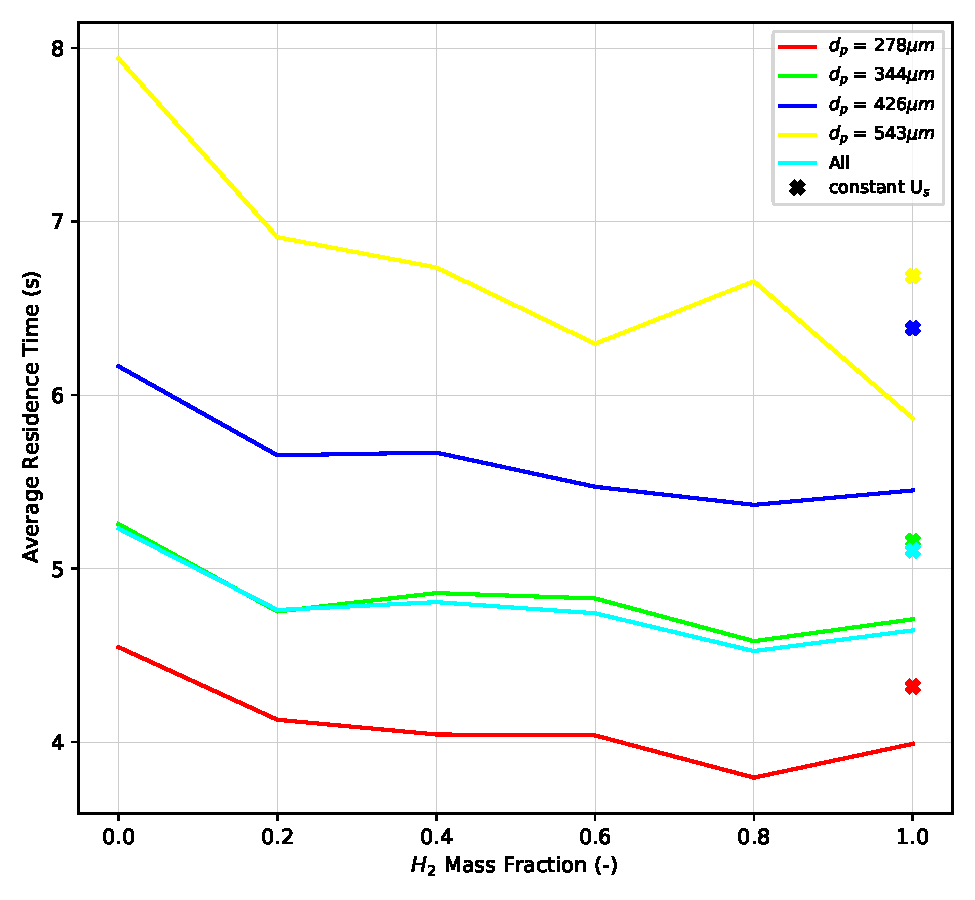
\includegraphics[width=0.8\textwidth]{figures/cfd-constuumf-rtd.pdf}
    \caption{Average particle residence time as a function of H$_2$ mass fraction in fluidizing gas at constant U$_\text{s}$/U$_\text{mf}$. Average residence times for H$_2$ fluidizing gas with constant U$_\text{s}$ indicated by markers in the plot.}
    \label{fig:cfd-constuumf-rtd}
\end{figure}

The effect of maintaining a constant U$_\text{s}$/U$_\text{mf}$ while increasing the mass fraction of H$_2$ in the fluidizing gas can be seen in Figure \ref{fig:cfd-constuumf-yields}, which contains plots of the product yields as well as the fraction of biomass converted for each gas composition and particle size. Because the particles must undergo significant mass loss and shrinkage before their terminal velocity is sufficiently low for elutriation, $>$99\% of the biomass is converted for all particle sizes and H$_2$ mass fractions investigated. For all particle sizes, the yields of light gasses and char decreased with increasing H$_2$ mass fraction with averages decreasing from 14.5\% to 13.3\% and 12.0\% to 10.6\%, respectively. These decreases in the char and light gas yields are accompanied by increases in the bio-oil yields, with the average increasing from 72.8\% in N$_2$ to 75.2\% in H$_2$. This increase is due to the low density of H$_2$ allowing for larger gas velocities without reducing the partice residence times. By maintaining similar residence times, the fraction of biomass converted to bio-oil remains constant while the higher gas velocities reduce the residence time of the resulting oil. The shorter residence time of the oil reduces the amount lost to secondary reactions converting it to char (repolymerization) and light gas (cracking). This can be seen in Figure \ref{fig:cfd-constuumf-reaction-rates} which shows the time and volume averaged cracking and repolymerization reaction rates in the reactor for each H$_2$ mass fraction. While maintaining a constant gas velocity when switching the fluidizing gas from N$_2$ to H$_2$ results in a slight increase in both secondary reactions, increasing the gas flowrate to maintain a constant U$_\text{s}$/U$_\text{mf}$ leads a decrease of 42.9\% in both the polymerization and cracking reaction rates. This results to the increased bio-oil production and subsequent decrease in light gas and char production when using H$_2$ as the fluidizing gas.

\begin{figure}[H]
    \centering
    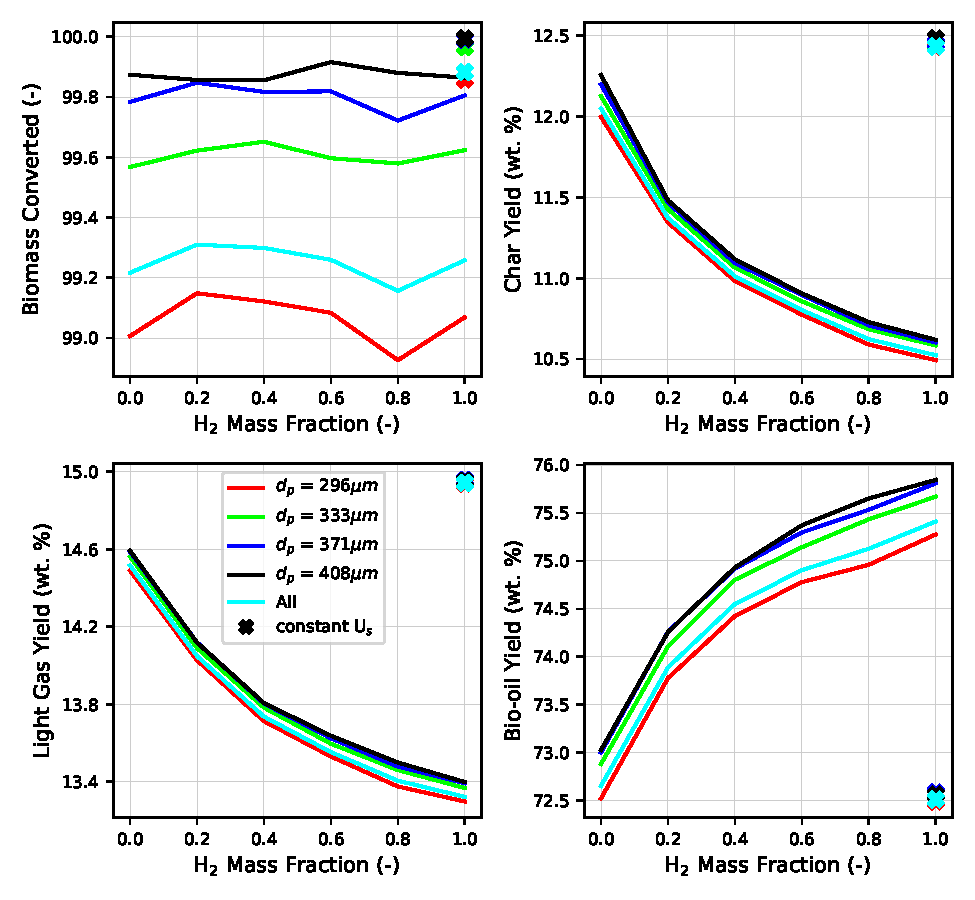
\includegraphics[width=\textwidth]{figures/cfd-constuumf-yields.pdf}
    \caption{Fraction of biomass converted and product yields as a function of H$_2$ mass fraction at constant U$_\text{s}$/U$_\text{mf}$. Biomass converted and product yields for H$_2$ fluidizing gas with constant U$_\text{s}$ indicated by markers in the plot.}
    \label{fig:cfd-constuumf-yields}
\end{figure}

\begin{figure}[H]
    \centering
    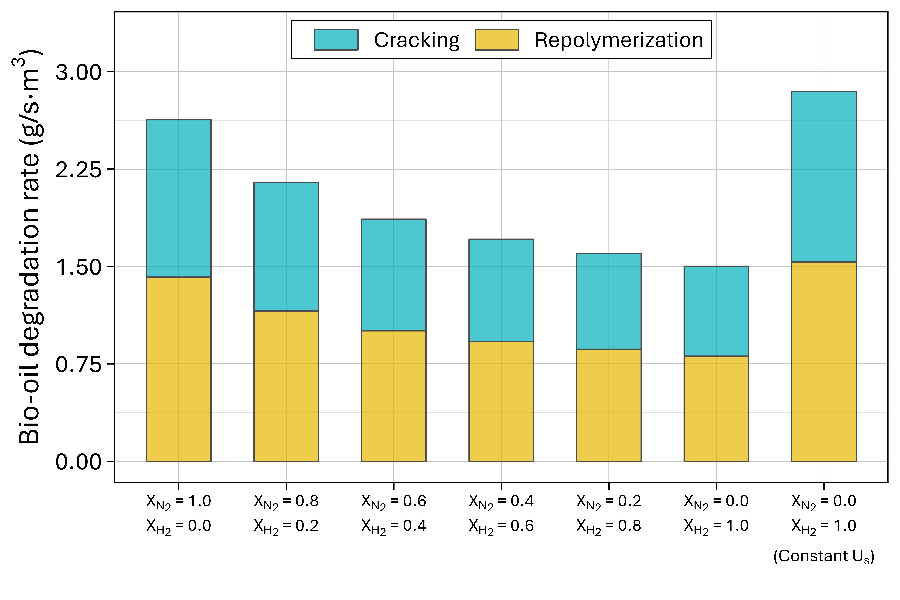
\includegraphics[width=1.0\textwidth]{figures/cfd-constuumf-reaction-rates.pdf}
    \caption{Volume and time averaged secondary reaction rates as a function of H$_2$ mass fraction at constant U$_\text{s}$/U$_\text{mf}$. Reaction rates with H$_2$ fluidizing gas and constant U$_\text{s}$ included for comparison.}
    \label{fig:cfd-constuumf-reaction-rates}
\end{figure}

% Conclusion
% ----------------------------------------------------------------------------

\section{Conclusion}

Gas effects in a fluidized bed biomass pyrolysis reactor using engineering correlations, low-order models, and CFD simulations were investigated for N$_2$, H$_2$, H$_2$O, CO, CO$_2$, and CH$_4$ carrier gas mixtures. Our findings reveal the importance of evaluating models and correlations for determining properties of a gas mixture. Two of the gas mixture models available in the literature (Brokaw as well as Herning \& Zipperer) compared well to experimental viscosity data. This contradicts results reported by Davidson who does not recommend the Herning and Zipperer method for hydrogen gas mixtures. The models from Davidson, Graham, and Wilke significantly underestimate the viscosity of the hydrogen mixtures investigated in this paper.

Fluidization characteristics and gas-solid heat transfer in a bubbling fluidized bed reactor can be greatly affected by the carrier gas properties. Based on our results, hydrogen gas requires approximately twice the flow rate of nitrogen gas to reach similar fluidization conditions in a BFB reactor. We also found that the thermal properties of the hydgrogen gas improves its convective heat transfer capability thus increasing its potential to pyrolyze biomass compared to a nitrogen gas environment. From our simulations, we found that the yield of bio-oil is independent of the carrier gas mixture when the flow rate is constant, with the average tar yield varying less than 2\% across each of the mixtures investigated. \textcolor{blue}{Furthermore, the utilization of H$_2$ as the fluidizing gas, while maintaining a constant U$_\text{s}$/U$_\text{mf}$, was shown to increase the bio-oil yields by $\sim$5\% when compared to the use of N$_2$.} This is due to the lower density H$_2$ producing similar hydrodynamics as N$_2$ at higher gas flowrates. These higher flowrates result in shorter gas residence times, and as a result, less secondary reactions converting bio-oil to light gases and char.

% Source code
% ----------------------------------------------------------------------------

\section{Source code}

Python code for calculating gas properties, fluidization characteristics, and for evaluating the pyrolysis kinetics is available on GitHub at \url{https://github.com/wigging/gas-effects-paper}. Functionality provided by the Chemics package was used for gas property and fluidization calculations. More information about Chemics is available at \url{https://chemics.github.io}.

% Acknowledgments
% ----------------------------------------------------------------------------

\section{Acknowledgments}

We thank the US Department of Energy’s (DOE) Bioenergy Technologies Office (BETO) for funding and supporting this work through the Feedstock-Conversion Interface Consortium (FCIC). This article used resources of the Compute and Data Environment for Science (CADES) at the Oak Ridge National Laboratory, which is supported by the Office of Science of the U.S. Department of Energy under Contract No. DE-AC05-00OR22725. This manuscript has been authored by UT-Battelle, LLC, under contract DE-AC05-00OR22725 with the US Department of Energy (DOE). The US government retains and the publisher, by accepting the article for publication, acknowledges that the US government retains a nonexclusive, paid-up, irrevocable, worldwide license to publish or reproduce the published form of this manuscript, or allow others to do so, for US government purposes. DOE will provide public access to these results of federally sponsored research in accordance with the DOE Public Access Plan (http://energy.gov/downloads/doe-public-access-plan).

% Supplemental material
% ----------------------------------------------------------------------------

\section{Supplemental material}

\textcolor{blue}{Gas density is calculated using the ideal gas law as shown in Equation \ref{eq:density} where $\rho_\text{gas}$ is density (kg/m$^3$), P is pressure (Pa), M is molecular weight (g/mol), R is the gas constant (m$^3\cdot$Pa / K$\cdot$mol), and T is temperature (K).}

\begin{equation}\label{eq:density}
    \rho_\text{gas} = \frac{P\,M}{R\,T}
\end{equation}

\textcolor{blue}{Molecular weight, viscosity, density, thermal conductivity, heat capacity, and the Prandtl number of the individual gases investigated in this paper are shown in Figure \ref{fig:gas-properties}. The gas properties were calculated at a pressure of 101,325 Pa and a temperature of 773.15 K (500$^\circ$C). The lightest gas in terms of molecular weight and density is hydrogen while the heaviest gas is carbon dioxide. The highest viscosity is noted for the nitrogen gas while hydrogen has the lowest viscosity. The largest thermal conductivity is for hydrogen at approximately 0.36 W/m$\cdot$K while the other gases remain below 0.12 W/m$\cdot$K. The highest heat capacity is obtained for methane at 62 J/mol$\cdot$K while the lowest is for hydrogen at 29 J/mol$\cdot$K. The Prandtl number is similar for all the gases except for water vapor.}

\begin{figure}[H]
    \centering
    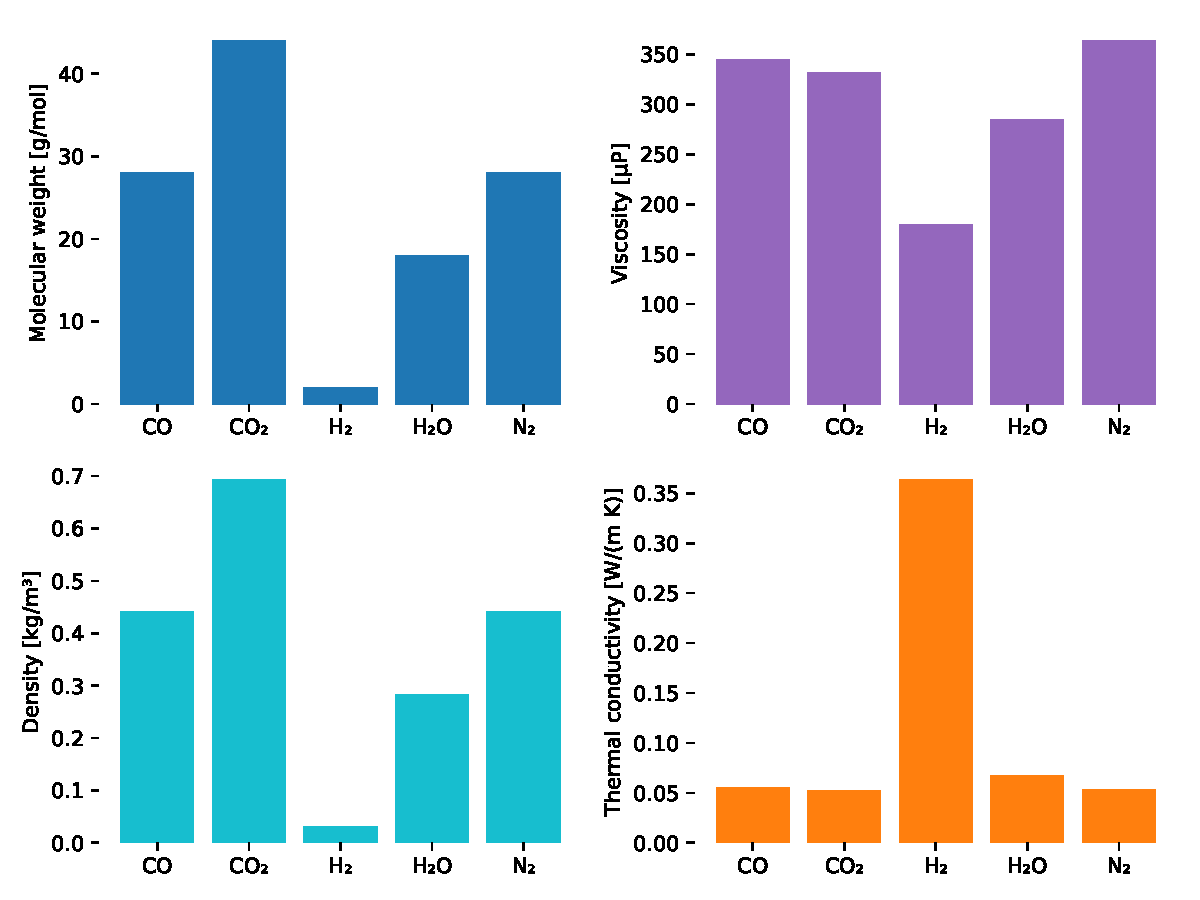
\includegraphics[width=\textwidth]{gas-properties.pdf}
    \caption{Comparison of molecular weight (MW), viscosity ($\mu$), density ($\rho$), thermal conductivity (k), heat capacity (Cp), and Prandtl number (Pr) for each gas at 101,325 Pa and 773.15 K (500$^\circ$C).}
    \label{fig:gas-properties}
\end{figure}

The Di Blasi kinetics were put to use in a batch reactor model to investigate the time scales associated with the reaction mechanisms. Figure \ref{fig:batch-blasi} is an overview of the biomass conversion and pyrolysis yields using the Di Blasi kinetics in a batch reactor at 773.15 K (500$^\circ$C). At this temperature, without the effects of secondary reactions, the kinetics offer a maximum achievable tar yield of 78\% within 5 seconds. However, if secondary reactions occur during the entire pyrolysis process then a maximum tar yield of only 53\% is possible. Modifying the pre-factor term for reaction 4 by a factor of 0.2, decreases the gas yield while increasing tar and char yields. The Di Blasi kinetics suggest that minimizing the extent of secondary reactions is critical to producing the maximum possible tar yield.

A range of reaction temperatures were applied to the Di Blasi kinetics in the batch reactor model as shown in Figure \ref{fig:batch-blasi-temps}. The kinetics suggest that temperature can increase the rate of primary tar production while decreasing devolatilization time. When secondary reactions occur during the entire pyrolysis process, maximum tar yields are realized at higher temperatures but with shorter residence times. These results suggest that if secondary reactions are minimized then maximum tar yield can be achieved within an appropriate residence time.

\begin{figure}[H]
    \centering
    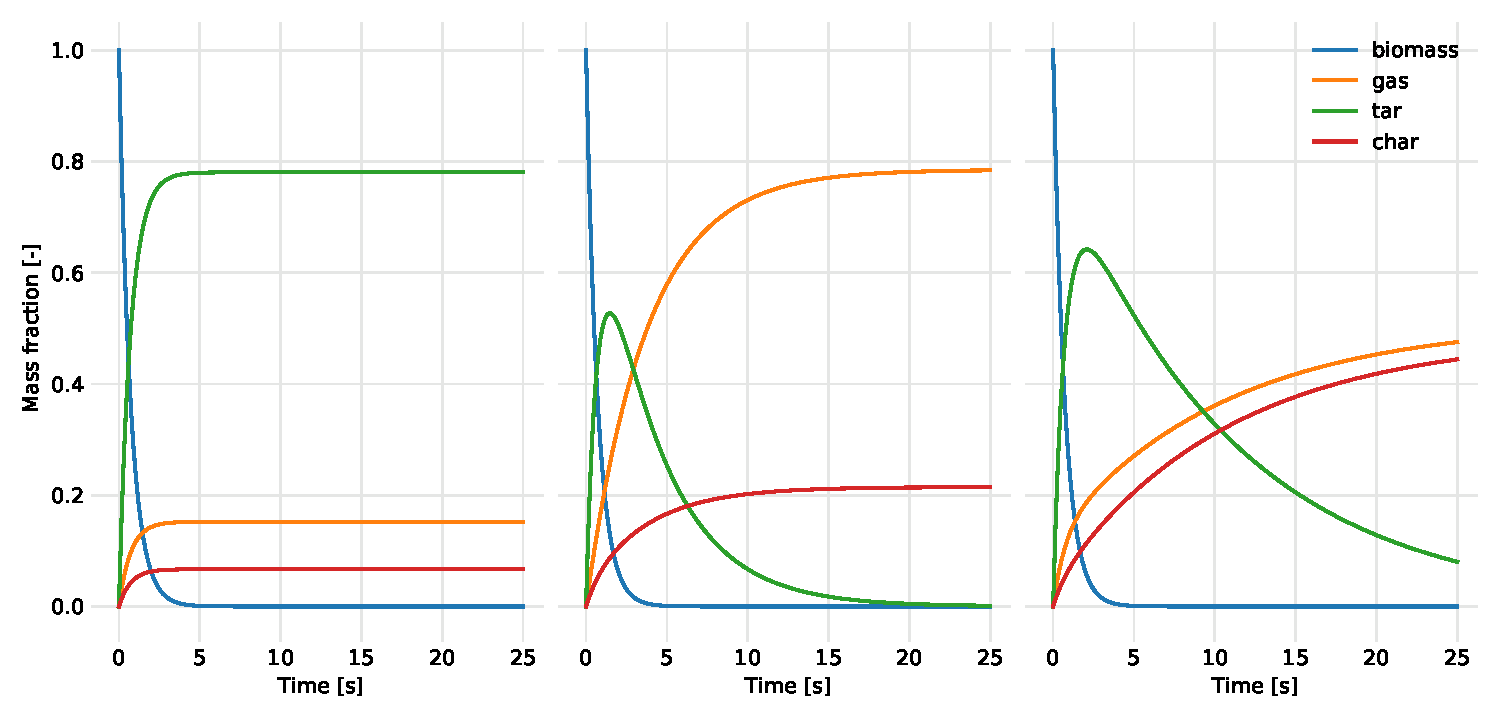
\includegraphics[width=\textwidth]{batch-blasi.pdf}
    \caption{Biomass conversion and product yields in a batch reactor model at 773.15 K (500$^\circ$C) according to the Di Blasi kinetic reactions. Primary reactions only (left). Primary and secondary reactions (center). Primary and secondary reactions using modified reaction 4 (right).}
    \label{fig:batch-blasi}
\end{figure}

\begin{figure}[H]
    \centering
    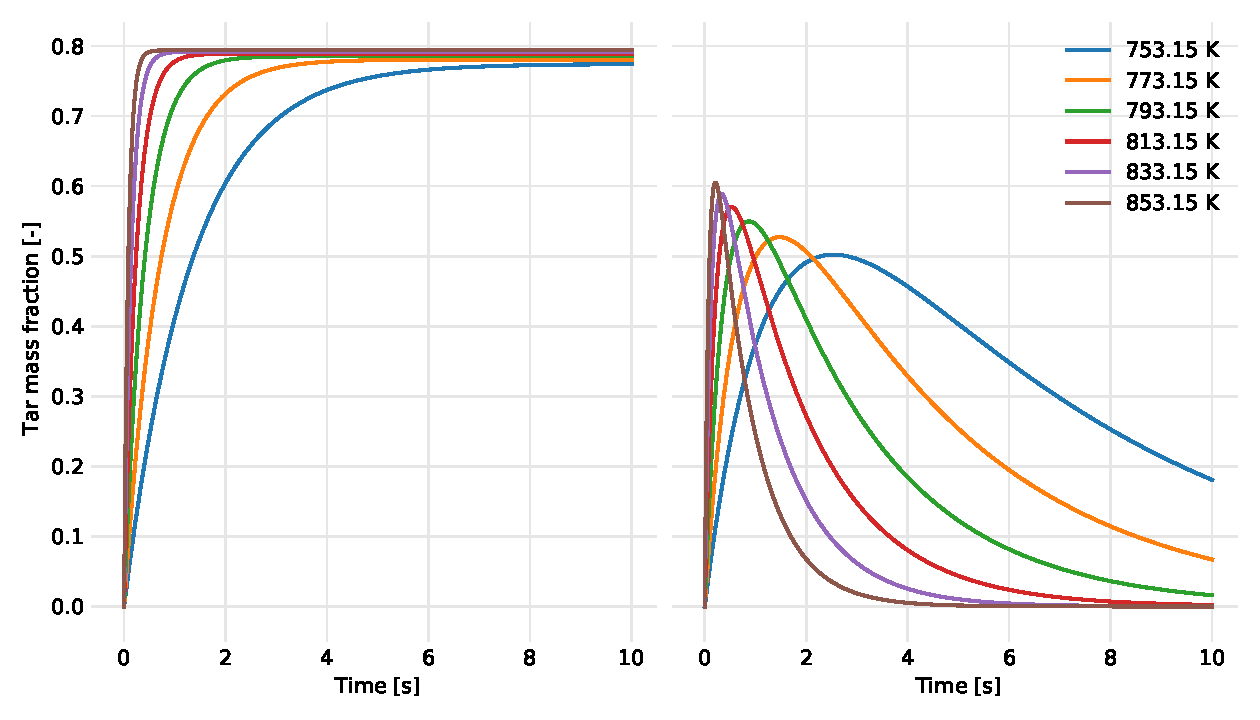
\includegraphics[width=\textwidth]{batch-blasi-temps.pdf}
    \caption{Tar yields for reaction temperatures of 753.15--853.15 K (480--580$^\circ$C) using the Di Blasi kinetics in a batch reactor model. Results shown for primary tar (left) along with primary and secondary tar (right).}
    \label{fig:batch-blasi-temps}
\end{figure}

% References
% ----------------------------------------------------------------------------

\printbibliography

\end{document}
